% \documentclass[11pt, oneside]{article}      % use "amsart" instead of "article" for AMSLaTeX format


\documentclass[submission,copyright,creativecommons]{eptcs}
\providecommand{\event}{QPL 2021}

% \usepackage{geometry}                       % See geometry.pdf to learn the layout options. There are lots.
% \geometry{letterpaper}                          % ... or a4paper or a5paper or ... 
%\geometry{landscape}                       % Activate for rotated page geometry
%\usepackage[parfill]{parskip}          	% Activate to begin paragraphs with an empty line rather than an indent
\usepackage{graphicx}
\usepackage{amsmath,amsthm,amssymb}
\usepackage{mathtools}
\usepackage{xcolor}
\usepackage[font=small,labelfont=bf,skip=0pt,justification=justified]{caption}
\usepackage{stackengine}
% \usepackage{natbib}
\usepackage{stmaryrd}
\usepackage[most]{tcolorbox}
\usepackage{tikzit}
\input{zx.tikzdefs}
\input{zx.tikzstyles}

\usepackage{hyperref} % must be last package used

% \bibliographystyle{abbrvnat}
% \setcitestyle{square, authoryear}
% \setlength{\parindent}{0in}
% \setcitestyle{square}
\theoremstyle{definition}
\newtheorem{theorem}{Theorem}[section]
\newtheorem{corollary}[theorem]{Corollary}
\newtheorem{lemma}[theorem]{Lemma}
\newtheorem*{lemma*}{Lemma}
\newtheorem*{proposition*}{Proposition}
\newtheorem{proposition}[theorem]{Proposition}
\newtheorem{conjecture}[theorem]{Conjecture}
\newtheorem{definition}[theorem]{Definition}
\newtheorem{example}[theorem]{Example}
\newtheorem{remark}[theorem]{Remark}
\newtheorem{warning}[theorem]{Warning}

\newcommand{\defeq}{\vcentcolon=}
\newcommand{\eqdef}{=\vcentcolon}
\newcommand{\xeq}[1]{\mathrel{\stackon[5pt]{$=$}{$\scriptstyle{#1}$}}}
\newcommand{\xeqq}[2]{\mathrel{\stackon[5pt]{$=$}{\stackon[5pt]{$\scriptstyle{#1}$}{$\scriptstyle{#2}$}}}}
\newcommand{\abs}[1]{\ensuremath{\lvert #1 \rvert}}

\newcommand{\qutritZphase}[2]{\,\tikz{\node[style=qutrit Z phase] (x) {$#1$ \nodepart{lower} $#2$};}\,}
\newcommand{\qutritXphase}[2]{\,\tikz{\node[style=qutrit X phase] (x) {$#1$ \nodepart{lower} $#2$};}\,}

\newcommand{\qutritZspider}[2]{\,\begin{tikzpicture}
	\begin{pgfonlayer}{nodelayer}
		\node [style=none] (1) at (0, 0.75) {...};
		\node [style=none] (5) at (-0.75, 1) {};
		\node [style=none] (7) at (0.75, 1) {};
		\node [style=none] (8) at (0, -0.75) {...};
		\node [style=none] (9) at (-0.75, -1) {};
		\node [style=qutrit Z phase] (10) at (0, 0) {$#1$ \nodepart{lower} $#2$};
		\node [style=none] (11) at (0.75, -1) {};
	\end{pgfonlayer}
	\begin{pgfonlayer}{edgelayer}
		\draw [bend left=15] (10) to (11.center);
		\draw [bend right=15] (10) to (9.center);
		\draw [bend right=15] (10) to (7.center);
		\draw [bend left=15] (10) to (5.center);
	\end{pgfonlayer}
\end{tikzpicture}}
\newcommand{\qutritState}[3]{\, \begin{tikzpicture}
	\begin{pgfonlayer}{nodelayer}
		\node [style=none] (1) at (0, 0.75) {};
		\node [style=qutrit #1 phase] (2) at (0, -0.5) {$#2$ \nodepart{lower} $#3$};
	\end{pgfonlayer}
	\begin{pgfonlayer}{edgelayer}
		\draw (1.center) to (2);
	\end{pgfonlayer}
\end{tikzpicture}}
\newcommand{\qutritZstate}[2]{\qutritState{Z}{#1}{#2}}
\newcommand{\qutritXstate}[2]{\qutritState{X}{#1}{#2}}

\newcommand{\qubitPhaseGate}[2]{\,\begin{tikzpicture}
	\begin{pgfonlayer}{nodelayer}
		\node [style=#1 phase dot] (0) at (0, 0) {$#2$};
		\node [style=none] (1) at (0, 1) {};
		\node [style=none] (2) at (0, -1) {};
	\end{pgfonlayer}
	\begin{pgfonlayer}{edgelayer}
		\draw (1.center) to (2.center);
	\end{pgfonlayer}
\end{tikzpicture}}
\newcommand{\qubitZphase}[1]{\qubitPhaseGate{Z}{#1}}
\newcommand{\qubitXphase}[1]{\qubitPhaseGate{X}{#1}}

\newcommand{\someSpider}[1]{$\mathcal{#1}$-spider}
\newcommand{\someSpiders}[1]{\someSpider{#1}s}
\newcommand{\Mspider}[0]{\someSpider{M}}
\newcommand{\Nspider}[0]{\someSpider{N}}
\newcommand{\Pspider}[0]{\someSpider{P}}
\newcommand{\Mspiders}[0]{\someSpiders{M}}
\newcommand{\Nspiders}[0]{\someSpiders{N}}
\newcommand{\Pspiders}[0]{\someSpiders{P}}

\newcommand{\smallcolvec}[1]{\ensuremath{\begin{psmallmatrix}#1\end{psmallmatrix}}}

\newcommand{\qutritRuleFusion}{\hyperlink{qutrit_rule_fusion}{\mathbf{(f)}}}
\newcommand{\qutritRuleId}{\hyperlink{qutrit_rule_id}{\mathbf{(id)}}}
\newcommand{\qutritRuleTwist}{\hyperlink{qutrit_rule_twisted_cup}{\mathbf{(t)}}}
\newcommand{\qutritRuleZeroCopy}{\hyperlink{qutrit_rule_0_copy}{\mathbf{(cp_0)}}}
\newcommand{\qutritRuleBialgebra}{\hyperlink{qutrit_rule_bialgebra}{\mathbf{(b)}}}
\newcommand{\qutritRuleMCopy}{\hyperlink{qutrit_rule_m_copy}{\mathbf{(cp_{\mathcal{M}})}}}
\newcommand{\qutritRuleCommute}{\hyperlink{qutrit_rule_commute}{\mathbf{(cm)}}}
\newcommand{\qutritRuleHadamard}{\hyperlink{qutrit_rule_hadamard}{\mathbf{(H)}}}
\newcommand{\qutritRuleEuler}{\hyperlink{qutrit_rule_euler}{\mathbf{(E)}}}
\newcommand{\qutritRuleColourChange}{\hyperlink{qutrit_rule_colour_change}{\mathbf{(cc)}}}
\newcommand{\qutritRuleSnake}{\hyperlink{qutrit_rule_snake}{\mathbf{(s)}}}

\newcommand{\qubitRuleFusion}{\hyperlink{qubit_rule_fusion}{\mathbf{(f)}}}
\newcommand{\qubitRuleId}{\hyperlink{qubit_rule_id}{\mathbf{(id)}}}
\newcommand{\qubitRuleCopy}{\hyperlink{qubit_rule_copy}{\mathbf{(c)}}}
\newcommand{\qubitRulePi}{\hyperlink{qubit_rule_pi}{(\bf{\pi})}}
\newcommand{\qubitRuleBialgebra}{\hyperlink{qubit_rule_bialgebra}{\mathbf{(b)}}}
\newcommand{\qubitRuleHadamard}{\hyperlink{qubit_rule_hadamard}{\mathbf{(H)}}}
\newcommand{\qubitRuleColourChange}{\hyperlink{qubit_rule_colour_change}{\mathbf{(cc)}}}
\newcommand{\qubitRuleEuler}{\hyperlink{qubit_rule_euler}{\mathbf{(E)}}}

\title{Classifying Complexity with the ZX Calculus}

\author{  Alex Townsend-Teague $^{0,1}$ and Konstantinos Meichanetzidis $^{1,2}$
\institute{$^0$ Mathematical Institute, University of Oxford}
\institute{$^1$ Department of Computer Science, University of Oxford}
\institute{$^2$ Cambridge Quantum Computing Ltd.} }

\def\titlerunning{Classifying Complexity with the ZX Calculus}
\def\authorrunning{Alex Townsend-Teague, Konstantinos Meichanetzidis}


\begin{document}
\maketitle
\begin{abstract}
The ZX calculus is a graphical language which allows for reasoning about suitably represented tensor networks, aka ZX diagrams,
in terms of rewrite rules.
Here, we focus on problems which amount to exactly computing
a scalar encoded as a closed tensor network.
In general, such problems are \#P-hard.
However, there are families of such problems which are known to be in P
when the dimension is bellow a certain value.
By expressing problem-instances from these families as ZX diagrams,
we see that the easy instances belong to the stabiliser fragment of the ZX calculus.
Building on previous work on efficient simplification of qubit stabiliser diagrams, we present simplifying rewrites for the case of qutrits.
Finally, we look at the specific examples of evaluating the Jones polynomial
and of counting graph-colourings.
Our exposition further constitutes the ZX calculus as a suitable and unifying language for studying the complexity of
a broad range of classical or quantum problems.
\end{abstract}

\section{Introduction}


A plethora of hard problems of interest to physics and computer science
regard interacting many-body multi-state systems, classical or quantum,
and reduce to \emph{exactly} computing a single scalar.
These range from probability amplitudes in quantum mechanics,
partition functions in classical statistical mechanics,
counting problems, probabilistic inference, and many more.
Problem instances can be encoded as a \emph{closed}
tensor-networks over an appropriate (semi)ring.
The scalar can be evaluated by \emph{full tensor contraction},
which in general is \#P-hard \cite{Damm2002}.
In fact, finding the optimal contraction path for a general tensor network is NP-hard.

The ZX calculus is a graphical language whose origin lies in the field of quantum foundations \cite{Coecke2011}.
It allows for reasoning about ZX diagrams, i.e. tensor networks which are expressed in terms of primitive generators \cite{vandewetering2020zxcalculus}.
The generators have a concrete representation as tensors over
a (semi)ring and they obey a set of rewrite rules which respect semantics \cite{wang2020completeness}.
Importantly, the rewrite rules \emph{depend} on the (semi)ring over which the diagram is interpreted as a tensor network.
If a scalar of interest is expressed as a ZX diagram,
one can rewrite the diagram by applying rewrite rules.
One's goal is then to apply a sequence of rewrites and perform \emph{full diagram simplification} in order to compute the desired scalar.
%Again, simplifying arbitrary closed ZX diagrams is \#P-hard and finding the optimal rewrite strategy is NP-hard.
Note that
given an arbitrary tensor network, one can attempt to invent rewrite rules by inspecting the contents of the tensors and performing linear-algebra operations \cite{gray2020hyperoptimized}.

In the context of quantum computing,
the Gottesman-Knill theorem states that stabiliser (or Clifford) circuits can be
simulated \emph{efficiently} on classical computers \cite{Aaronson2004}.
By simulation here we mean the \emph{exact} computation of \emph{amplitudes}.
These circuits are can be expressed by the \emph{stabiliser} fragment of the ZX calculus.
An alternative, and in fact more general, proof of the Gottesman-Knill theorem for qubits has been obtained graphically in terms of the qubit ZX calculus.
Interestingly, even if the motivation for studying stabiliser diagrams stems from quantum computation, the result that stabiliser ZX diagrams can be simplified efficiently has broader applicability. This is because
ZX diagrams can express arbitrary linear maps; not every ZX diagram is a quantum circuit, but every quantum circuit can be cast as a ZX diagram.

Beyond quantum computing, ZX diagrams have been leveraged to study the complexity of boolean satisfiability (SAT) and model counting (\#SAT) \cite{debeaudrap2020tensor}.
Model counting entails computing the number of satisfying assignments to a boolean formula (which is given in conjunctive normal form)
and this number can be expressed a closed diagram.
Specifically, one finds that in the case of XORSAT and \#XORSAT,
which are known to be tractable,
the corresponding ZX diagrams representing the problems exactly correspond to qubit stabilizer diagrams, which are efficient to simplify.
Going further, the ZH calculus \cite{backens2018zh}, an extension of the ZX calculus, can be imported to make graphically obvious
why 2SAT is in P but \#2SAT is \#P-complete while 3SAT is NP-complete and \#3SAT is \#P-hard.
That is, the counting version of 2SAT is hard while deciding is easy, but this is not the case for 3SAT where both deciding and counting are hard.
The \emph{key realisation} is in that the decision problem is a counting problem
but where the diagram is interpreted over the Boolean semiring.
% (where $1+1=2$).
Then the \emph{rewrite rules change accordingly} and obviously imply the above result by allowing efficient simplification strategies.

Such observations make apparent the \emph{unifying power of diagrammatic reasoning
for studying the complexity} of problem families of universal interest,
where the degrees of freedom are two-dimensional.
Building on the spirit of \cite{debeaudrap2020tensor}, we treat ZX as a library comprising out-of-the-box and readily-available diagrammatic rewrite-rules from which we import the appropriate tools for the job depending on the occasion.
The key rewrite rules that enable the efficient diagram simplification
of qubit stabiliser ZX diagrams
are called \emph{local complementation} and \emph{pivot},
the latter being composition of three of the former \cite{graph_theoretic_simplification}.
In this work, we recall the qutrit version of local complementation and derive the corresponding pivot rule
which implies that qutrit stabiliser diagrams can be simplified efficiently.
We then present two case studies: evaluating the Jones polynomial at lattice roots of unity, and graph colouring.
Both of these problem families reduce to evaluating
closed tensor networks and show a transition in complexity
at a particular dimension, bellow which the tensor network corresponds to a stabiliser ZX diagram.

We underline that throughout this work, all rewrites are valid
\emph{up to scalar}
since we are only concerned about making statements about complexity.

% % \section{From a Link to a ZX-Diagram}

We begin by describing the passage from a link $L$ to a ZX-diagram $D$ which represents the evaluation of the Jones polynomial of $L$ at lattice roots of unity. The majority of this journey is as detailed in \cite{jones_tensors}, though the final small step into the ZX-calculus is new. This section aims to be comprehensible to those with no background in topology or statistical mechanics; we introduce only as many terms as needed to describe the passage fully, keeping definitions simple and providing several figures. After this first jargon-heavy section, we will be working almost exclusively in a ZX setting.\newline

We will define a knot $K$ to be a circle smoothly embedded in $\mathbb{R}^3$. More generally, an \textit{n-component link} $L$ will be a smooth embedding of $n$ disjoint circles in $\mathbb{R}^3$. A \textit{link diagram} for $L$ is a projection of the link onto some plane in $\mathbb{R}^3$ but with over- and undercrossing information retained. Thus a given link has infinitely many link diagrams. Intuitively, a link diagram is what one produces when one attempts to draw a link in two dimensions. An \textit{oriented link} has a direction assigned to each component knot; this is indicated in a link diagram by an arrow. As an example, we show diagrams for two different orientations of the trefoil knot linked with an unknot:\newline

[Insert diagram]\newline

Two oriented links $L$ and $L'$ are isotopic, written $L \simeq L'$, if and only if there is a finite sequence of \textit{Reidemeister moves} taking a diagram for $L$ to a diagram for $L'$. These moves, shown in Appendix [ToDo ref], precisely capture the notion of reversible local strand deformations that do not change the topology. For example, they do not permit breaking or gluing of strands, passing one strand through another, or reversing of orientations. The \textit{Jones polynomial} $V_L(z)$ for an oriented link $L$ is a polynomial in $z \in \mathbb{C}$. It is a \textit{link invariant}; that is, $V_L(z) \neq V_{L'}(z)$ implies $L \not\simeq L'$, for any two oriented links $L$ and $L'$. In general, computing $V_L(z)$ is exponentially costly in the number $\abs{C}$ of crossings of $L$, but it is known that at the special cases of the \textit{lattice roots of unity} $z \in \{\pm 1, \pm i, \pm e^{i\frac{2\pi}{3}}, \pm e^{i\frac{4\pi}{3}}\}$ it can be evaluated in time polynomial in $\abs{C}$ [Welsh]:\newline

[Draw lattice roots of unity]\newline

Let $z_q = \frac{1}{2}\left(q - 2 + \sqrt{q(q - 4)}\right)$, and note the correspondence $(z_1, z_2, z_3, z_4) = (e^{i\frac{2\pi}{3}}, i, e^{i\frac{\pi}{3}}, 1)$ with the lattice roots of unity. Remarkably, the Jones polynomial $V_L(z_q)$ at the points $q \in \{1, 2, 3, 4\}$ can be expressed in terms of the \textit{partition function} $Z(q)$ of a \textit{$q$-state Potts model} [Wu]. For those with no statistical mechanical background, given some graph $G = (V, E)$, a $q$-state Potts model on $G$ can just be thought of as the ability to assign a \textit{spin} $\sigma_v \in \{1, ..., q\}$ to each vertex $v \in V$, along with a partition function $Z: \{1, .., q\} \rightarrow \mathbb{C}$, which in physics usually captures some thermodynamical properties of a system. This function has an explicit formula in the general case, but it will make more sense to defer stating this until we have introduced enough terminology to give a simpler formula pertaining to our circumstances (see [ToDo] below). A particular assignment $\sigma = (\sigma_1, ..., \sigma_{\abs{V}})$ of spins to each vertex will be called a \textit{configuration}.\newline

In our case, we will define a Potts model on a particular \textit{signed graph} - a graph in which every edge has a positive or negative sign - called a \textit{Tait graph} of the link $L$. This is denoted $G_L = (V_L, E_L)$ and obtained as follows. First, an arbitrary link diagram for $L$ is given a \textit{checkerboard colouring}. That is, regions of $\mathbb{R}^2$ carved out by the link are shaded black or white such that no two adjacent regions have the same colour. For any diagram for $L$ there are exactly two equivalent ways to do this, the difference between the two just being that the roles of black and white are swapped throughout. Therefore we fix a convention that the unique unbounded region surrounding the link (i.e. the background) will be white.\newline

[Diagram]\newline

Next, every shaded (black) region is mapped to a vertex and every crossing is mapped to a signed edge $e = vw$ according to its orientation relative to the surrounding colours, per the rule shown in [ToDo] below. The signs $\varepsilon_{vw} = \pm$ of these edges are called \textit{Tait signs} and are graphically denoted by a small box on the corresponding edge, labelled with either a plus or minus sign appropriately. If we now define a Potts model on $G_L$, the partition function $Z(q)$ has the following formula. We sum over all possible configurations $\sigma$ of spins, and within each term we multiply together the values $-z_q^{-\varepsilon_{vw}}$ for all edges $vw$ whose endpoints have the same spin in this configuration. That is:

\begin{equation}
	Z(q) = \sum_{\sigma} \left( \prod_{vw \in E_L} T_{\sigma_v, \sigma_w}^{(q)} \right)
\end{equation}
\begin{equation}
	T_{\sigma_v, \sigma_{w}}^{(q)}
	= \begin{cases}
		-z_q^{-\varepsilon_{vw}} &\ \ \text{if} \ \ \sigma_v = \sigma_{w} \\  
		1 &\ \ \text{if} \ \ \sigma_v \neq \sigma_{w}
	\end{cases}
\end{equation}

For fixed $v, w$ we can view $T_{(-)_v,(-)_w}^{(q)} \eqdef T_{\varepsilon_{vw}}^{(q)}$ as a $q \times q$ matrix, indexed by the possible spins $\{1, ..., q\}$ that could be assigned to $v$ and $w$: 

\begingroup
	\renewcommand*{\arraystretch}{1.5}
	\begin{equation}
	T_{-_v,-_w}^{(q)}
	\begin{pmatrix}
		-z_q^{-\varepsilon_{vw}} & 1 & \dots & 1 \\
		1 & -z_q^{-\varepsilon_{vw}} & \dots & 1 \\
		\vdots & \vdots & \ddots & \vdots\\
		1 & 1  & \dots & -z_q^{-\varepsilon_{vw}}
	\end{pmatrix}
\end{equation}
\endgroup

Finally, the actual statement relating the Jones polynomial to the partition function is:

\begin{equation}
	V_L(z_q) = \mathcal{A}_L(q)Z(q)
\end{equation}

where $\mathcal{A}_L(q)$ is an efficiently computable prefactor, whose definition is given in Appendix [ToDo]. 
% For completeness, we give its formula, where $w(L)$ denotes the \textit{writhe} of the link $L$ [ToDo: ref], and the \textit{Tait number} $\tau(L)$ is the sum $\sum_{vw \in E_L} \varepsilon_{vw}$ of all the Tait signs:
% \begin{equation}
% 	\mathcal{A}_L(q) = (-z_q^{\frac{1}{2}} - z_q^{-\frac{1}{2}})^{-\abs{V_L} - 1}(-z_q^{\frac{3}{4}})^{w(L)}z_q^{\frac{1}{4}\tau(L)}
% \end{equation}

\begin{remark}
	Of course, different diagrams for $L$ will lead to different (non-isomorphic) Tait graphs $G_L$. Ultimately, however, this will not matter to us. This is because the Tait signs are related to $z_q$ in such a way that graph operations on $G_L$ corresponding to Reidemeister moves on $L$ leave $Z(q)$ (ToDo: and therefore $\mathcal{A}_L(q)$?) invariant [ToDo: ref].
	 % $\varepsilon_{vw} = \pm$ determine \textit{spin-spin interactions} $J_{\pm} = \text{[ToDo]}$, which are related to the variable $z_q$ of the Jones polynomial $V_L(z_q)$ via the equality $z_q = -e^{\mp J_\pm}$. As a result, it can be shown [ToDo ref] that the interactions $J_\pm$ are such that the graph operations on $G_L$ corresponding to Reidemeister moves on $L$ leave $Z(q)$ invariant. 
\end{remark}



% After defining a Potts model on the Tait graph $G_L$, every signed edge indicates a \textit{spin-spin Tait-sign-dependent interaction} $J_\pm \in \mathbb{C}$. These interactions relate to the variable $z$ of the Jones polynomial via the equality $z = -e^{\mp J_\pm}$. The role of the link invariant is played by the partition function $Z(q)$; in fact, the interactions $J_\pm$ are such that the graph operations on $G_L$ corresponding to Reidemeister moves on $L$ leave $Z(q)$ invariant. Specifically, $Z(q)$ is related to the Jones polynomial by $V_L(z) = \mathcal{A}_L(z)Z(q)$, where $A_L(z)$ is an efficiently computable value which handles bookeeping of twist factors [Definition?]. Its explicit definition is given in [ToDo] in the Appendix. has the following explicit formula: [Check again with Kon!]\newline






% For the case $q=3$ we use the qutrit ZX calculus:
% % \begin{equation}
% % 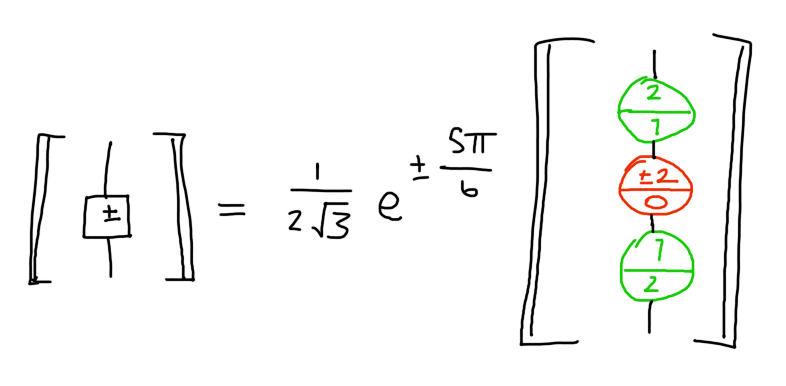
\includegraphics[scale=0.3]{figures/sketches/Qutrit Potts matrices.png}
% % \end{equation}

% For the case $q=4$ we are back again in the usual qubit ZX calculus:
% % \begin{equation}
% % 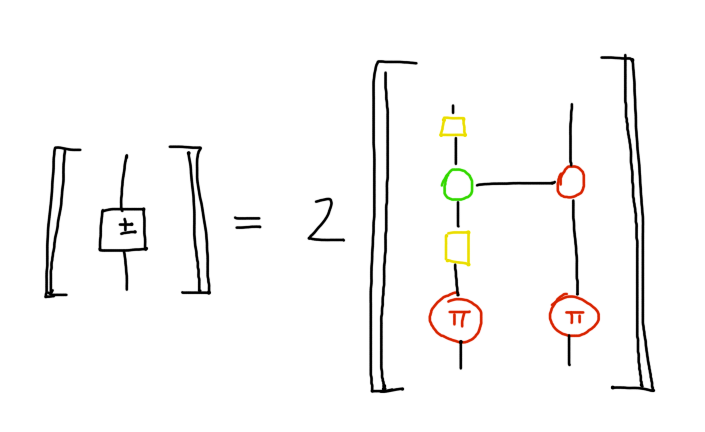
\includegraphics[scale=0.3]{figures/sketches/Qu(4)it Potts matrices.png}
% % \end{equation}

% In each case, the resulting map is in the stabilizer fragment of the ZX calculus. 
 
% \section{From a Link to a ZX-Diagram}\label{sec:passage}

We begin by describing the passage from a link $L$ to a ZX-diagram $D$ which represents the evaluation of the Jones polynomial of $L$ at lattice roots of unity. The majority of this journey is as detailed in \citep{jones_tensors}, though the final small step into the ZX-calculus is new. Since this section aims to be comprehensible to those with no background in topology or statistical mechanics, we leave most of the details to \citep{jones_tensors}. We introduce only as many terms as needed to describe the passage fully, keeping definitions simple and providing several figures. After this first jargon-heavy section, we will be working almost exclusively in a ZX setting.\newline

We will define an \textit{n-component link} $L$ to be a smooth embedding of $n$ disjoint circles in $\mathbb{R}^3$. A \textit{link diagram} for $L$ is a projection of the link onto some plane in $\mathbb{R}^3$ but with over- and undercrossing information retained. Thus a given link has infinitely many link diagrams. Intuitively, a link diagram is what one produces when one attempts to draw a link in two dimensions. An \textit{oriented link} has a direction assigned to each component; this is indicated in a link diagram by an arrow. As an example is shown below:\newline

[diagram]\newline

Two oriented links $L$ and $L'$ are isotopic, written $L \simeq L'$, if and only if there is a finite sequence of \textit{Reidemeister moves} [ToDo: ref] taking a diagram for $L$ to a diagram for $L'$. These moves precisely capture the notion of reversible local strand deformations that do not change the topology. For example, they do not permit breaking or gluing of strands, passing one strand through another, or reversing of orientations. The \textit{Jones polynomial} $V_L(z)$ for an oriented link $L$ is a polynomial in $z \in \mathbb{C}$. It is a \textit{link invariant}; that is, $V_L(z) \neq V_{L'}(z)$ implies $L \not\simeq L'$, for any two oriented links $L$ and $L'$. In general, computing $V_L(z)$ is exponentially costly in the number $\abs{C}$ of crossings of $L$, but it is known that at the special cases of the \textit{lattice roots of unity} $z \in \{\pm 1, \pm i, \pm e^{i\frac{2\pi}{3}}, \pm e^{i\frac{4\pi}{3}}\}$ it can be evaluated in time polynomial in $\abs{C}$ [Welsh]:\newline

[Draw lattice roots of unity]\newline

Now, for any diagram of a link $L$ there is an associated \textit{Tait graph}. This is denoted $G_L = (V_L, E_L)$ and obtained as follows. First, the link diagram is given a \textit{checkerboard colouring}. That is, regions of $\mathbb{R}^2$ carved out by the link are shaded black or white such that no two adjacent regions have the same colour. For any diagram for $L$ there are exactly two equivalent ways to do this, the difference between the two just being that the roles of black and white are swapped throughout. Therefore we fix a convention that the unique unbounded region surrounding the link (i.e. the background) will be white.\newline

[diagram]\newline

Next, every shaded (black) region is mapped to a vertex and every crossing is mapped to a signed edge $e = vw$ according the rule shown below. The signs $\varepsilon_{vw} = \pm$ of these edges are called \textit{Tait signs} and are graphically denoted by a small box on the corresponding edge, labelled with either a plus or minus sign appropriately:\newline

[diagram]\newline

If we now suppose that the vertices and Tait signs actually represent \textit{tensors} (multidimensional matrices), then this Tait graph above can be interpreted as a closed \textit{tensor network} in diagrammatic notation [ToDo: ref], which we'll denote $Z(q)$. In fact, suppose we let $z_q = \frac{1}{2}\left(q - 2 + \sqrt{q(q - 4)}\right)$, and let the vertices and Tait signs denote the following tensors:

\begingroup
	\renewcommand*{\arraystretch}{1.25}
	\begin{equation}\label{eq:pm_tensor}
		T_\pm^{(q)} = 
		\left\llbracket \ \tikzfig{pm_maps/pm} \ \right\rrbracket = 
		\begin{pmatrix}
			-z_q^{\mp 1} & 1 & \dots & 1 \\
			1 & -z_q^{\mp 1} & \dots & 1 \\
			\vdots & \vdots & \ddots & \vdots\\
			1 & 1 & \dots & -z_q^{\mp 1}
		\end{pmatrix}
	\end{equation}
	\begin{equation}\label{eq:vertex_tensor}
		\tilde{T}^{(q)} =
		\left\llbracket \ \ \tikzfig{pm_maps/vertex} \ \ \right\rrbracket = 
		\text{ToDo}
	\end{equation}
\endgroup

Then remarkably the resulting closed tensor network $Z(q)$ is equal to the Jones polynomial $V_L(z_q)$ at these specific points, up to a prefactor $\mathcal{A}_L(q)$ [ToDo: ref]. Computing this prefactor is known to be efficient, so if we can show that computing $Z(q)$ is also efficient then we'll have shown that computing $V_L(z_q)$ is efficient. Note the correspondence $(z_1, z_2, z_3, z_4) = (e^{i\frac{2\pi}{3}}, i, e^{i\frac{\pi}{3}}, 1)$ with the lattice roots of unity. 

\begin{remark}
	Of course, different diagrams for $L$ will lead to different (non-isomorphic) Tait graphs $G_L$. Ultimately, however, this will not matter to us. This is because the Tait signs $\varepsilon_{vw}$ are related to $z_q$ in such a way that graph operations on $G_L$ corresponding to Reidemeister moves on $L$ leave $Z(q)$ (ToDo: and $\mathcal{A}_L(q)$?) invariant [ToDo: ref].
\end{remark}

\begin{remark}
	$Z(q)$ is in fact the partition function of a $q$-state Potts model placed on the Tait graph $G_L$. [ToDo: say more?]
\end{remark}

In order to demonstrate efficient computability of $Z(q)$ for $q \in \{1, 2, 3, 4\}$, we will find representations for the tensors $T_\pm^{(q)}$ and $\tilde{T}^{(q)}$ in the \textit{ZX-calculus}, a graphical language for quantum mechanics based on $q$-dimensional qudits, introduced formally in the next two sections. For $q=1$ the calculus is trivial - there is exactly one $1$-dimensional qudit - so only the cases $q \in \{2, 3, 4\}$ remain. For $q=4$ the isomorphism $\mathbb{C}^4 \cong \mathbb{C}^2 \otimes \mathbb{C}^2$ means we can use the same 2-dimensional calculus as for $q=2$. We will soon see that both the 2-dimensional (\textit{qubit}) and 3-dimensional (\textit{qutrit}) ZX-calculus feature \textit{green spiders}, and in all three cases $q \in \{2, 3, 4\}$ these are the right choice of representative of the vertex tensor $\tilde{T}^{(q)}$.

\begin{proposition}\label{prop:vertex_tensor_Z_spider}
	The tensor represented by a vertex in the Tait graph is related (ToDo: how!?) to the \textit{standard interpretation} of the green spider in the cases $q \in \{2, 3, 4\}$.
	\begin{equation*}
		\tilde{T}^{(q)} \ = \ 
		\left\llbracket \ \ \tikzfig{pm_maps/vertex} \ \ \right\rrbracket \ \sim \ 
		\left\llbracket \ \ \tikzfig{pm_maps/z_spider} \ \ \right\rrbracket
	\end{equation*}
	\begin{proof}
		See Appendix [ToDo].
	\end{proof}
\end{proposition}

ZX-diagrams corresponding to the $q \times q$ matrix $T_\pm^{(q)}$ are given after the ZX-calculi have been properly introduced (Propositions \ref{prop:pm_map_q2_q4} and \ref{prop:pm_map_q3}). [ToDo: say more! Move discussion about scalar exactness here? Explain how contracting this tensor network/ZX-diagram means evaluating $Z(q)$?]


% Let $z_q = \frac{1}{2}\left(q - 2 + \sqrt{q(q - 4)}\right)$, and note the correspondence $(z_1, z_2, z_3, z_4) = (e^{i\frac{2\pi}{3}}, i, e^{i\frac{\pi}{3}}, 1)$ with the lattice roots of unity. Remarkably, the Jones polynomial $V_L(z_q)$ at the points $q \in \{1, 2, 3, 4\}$ can be expressed in terms of the \textit{partition function} $Z(q)$ of a \textit{$q$-state Potts model} [Wu]. 



% For those with no statistical mechanical background, given some graph $G = (V, E)$, a $q$-state Potts model on $G$ can just be thought of as the ability to assign a \textit{spin} $\sigma_v \in \{1, ..., q\}$ to each vertex $v \in V$, along with a partition function $Z: \{1, .., q\} \rightarrow \mathbb{C}$, which in physics usually captures some thermodynamical properties of a system. This function has an explicit formula in the general case, but it will make more sense to defer stating this until we have introduced enough terminology to give a simpler formula pertaining to our circumstances (see [ToDo] below). A particular assignment $\sigma = (\sigma_1, ..., \sigma_{\abs{V}})$ of spins to each vertex will be called a \textit{configuration}.\newline

% In our case, we will define a Potts model on a particular \textit{signed graph} - a graph in which every edge has a positive or negative sign - called a \textit{Tait graph} of the link $L$. This is denoted $G_L = (V_L, E_L)$ and obtained as follows. First, an arbitrary link diagram for $L$ is given a \textit{checkerboard colouring}. That is, regions of $\mathbb{R}^2$ carved out by the link are shaded black or white such that no two adjacent regions have the same colour. For any diagram for $L$ there are exactly two equivalent ways to do this, the difference between the two just being that the roles of black and white are swapped throughout. Therefore we fix a convention that the unique unbounded region surrounding the link (i.e. the background) will be white.\newline

% [Diagram]\newline

% Next, every shaded (black) region is mapped to a vertex and every crossing is mapped to a signed edge $e = vw$ according to its orientation relative to the surrounding colours, per the rule shown in [ToDo] below. The signs $\varepsilon_{vw} = \pm$ of these edges are called \textit{Tait signs} and are graphically denoted by a small box on the corresponding edge, labelled with either a plus or minus sign appropriately. If we now define a Potts model on $G_L$, the partition function $Z(q)$ has the following formula. We sum over all possible configurations $\sigma$ of spins, and within each term we multiply together the values $-z_q^{-\varepsilon_{vw}}$ for all edges $vw$ whose endpoints have the same spin in this configuration. That is:

% \begin{equation}
% 	Z(q) = \sum_{\sigma} \left( \prod_{vw \in E_L} T_{\sigma_v, \sigma_w}^{(q)} \right)
% \end{equation}
% \begin{equation}
% 	T_{\sigma_v, \sigma_{w}}^{(q)}
% 	= \begin{cases}
% 		-z_q^{-\varepsilon_{vw}} &\ \ \text{if} \ \ \sigma_v = \sigma_{w} \\  
% 		1 &\ \ \text{if} \ \ \sigma_v \neq \sigma_{w}
% 	\end{cases}
% \end{equation}

% For fixed $v, w$ we can view $T_{(-)_v,(-)_w}^{(q)} \eqdef T_{\varepsilon_{vw}}^{(q)}$ as a $q \times q$ matrix, indexed by the possible spins $\{1, ..., q\}$ that could be assigned to $v$ and $w$: 

% \begingroup
% 	\renewcommand*{\arraystretch}{1.5}
% 	\begin{equation}
% 	T_{-_v,-_w}^{(q)}
% 	\begin{pmatrix}
% 		-z_q^{-\varepsilon_{vw}} & 1 & \dots & 1 \\
% 		1 & -z_q^{-\varepsilon_{vw}} & \dots & 1 \\
% 		\vdots & \vdots & \ddots & \vdots\\
% 		1 & 1  & \dots & -z_q^{-\varepsilon_{vw}}
% 	\end{pmatrix}
% \end{equation}
% \endgroup

% Finally, the actual statement relating the Jones polynomial to the partition function is:

% \begin{equation}
% 	V_L(z_q) = \mathcal{A}_L(q)Z(q)
% \end{equation}

% where $\mathcal{A}_L(q)$ is an efficiently computable prefactor, whose definition is given in Appendix [ToDo]. 
% % For completeness, we give its formula, where $w(L)$ denotes the \textit{writhe} of the link $L$ [ToDo: ref], and the \textit{Tait number} $\tau(L)$ is the sum $\sum_{vw \in E_L} \varepsilon_{vw}$ of all the Tait signs:
% % \begin{equation}
% % 	\mathcal{A}_L(q) = (-z_q^{\frac{1}{2}} - z_q^{-\frac{1}{2}})^{-\abs{V_L} - 1}(-z_q^{\frac{3}{4}})^{w(L)}z_q^{\frac{1}{4}\tau(L)}
% % \end{equation}

% \begin{remark}
% 	Of course, different diagrams for $L$ will lead to different (non-isomorphic) Tait graphs $G_L$. Ultimately, however, this will not matter to us. This is because the Tait signs are related to $z_q$ in such a way that graph operations on $G_L$ corresponding to Reidemeister moves on $L$ leave $Z(q)$ (ToDo: and therefore $\mathcal{A}_L(q)$?) invariant [ToDo: ref].
% 	 % $\varepsilon_{vw} = \pm$ determine \textit{spin-spin interactions} $J_{\pm} = \text{[ToDo]}$, which are related to the variable $z_q$ of the Jones polynomial $V_L(z_q)$ via the equality $z_q = -e^{\mp J_\pm}$. As a result, it can be shown [ToDo ref] that the interactions $J_\pm$ are such that the graph operations on $G_L$ corresponding to Reidemeister moves on $L$ leave $Z(q)$ invariant. 
% \end{remark}



% After defining a Potts model on the Tait graph $G_L$, every signed edge indicates a \textit{spin-spin Tait-sign-dependent interaction} $J_\pm \in \mathbb{C}$. These interactions relate to the variable $z$ of the Jones polynomial via the equality $z = -e^{\mp J_\pm}$. The role of the link invariant is played by the partition function $Z(q)$; in fact, the interactions $J_\pm$ are such that the graph operations on $G_L$ corresponding to Reidemeister moves on $L$ leave $Z(q)$ invariant. Specifically, $Z(q)$ is related to the Jones polynomial by $V_L(z) = \mathcal{A}_L(z)Z(q)$, where $A_L(z)$ is an efficiently computable value which handles bookeeping of twist factors [Definition?]. Its explicit definition is given in [ToDo] in the Appendix. has the following explicit formula: [Check again with Kon!]\newline






% For the case $q=3$ we use the qutrit ZX calculus:
% % \begin{equation}
% % 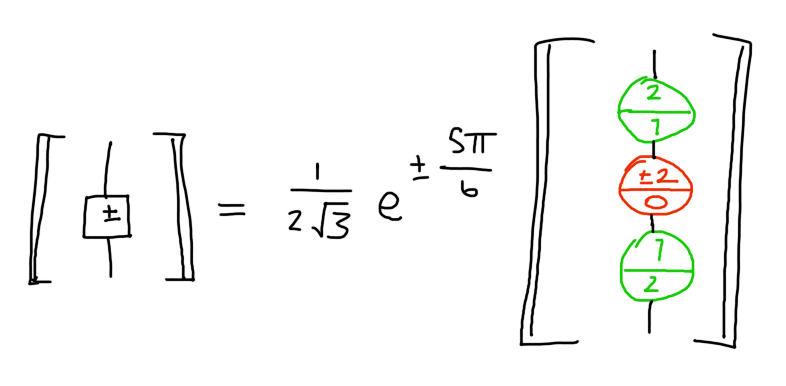
\includegraphics[scale=0.3]{figures/sketches/Qutrit Potts matrices.png}
% % \end{equation}

% For the case $q=4$ we are back again in the usual qubit ZX calculus:
% % \begin{equation}
% % 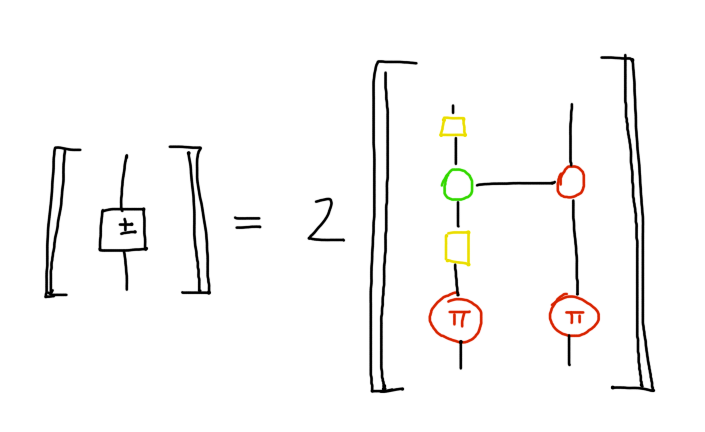
\includegraphics[scale=0.3]{figures/sketches/Qu(4)it Potts matrices.png}
% % \end{equation}

% In each case, the resulting map is in the stabilizer fragment of the ZX calculus. 
 

\section{Simplifying Qubit ZX-Diagrams}

In this section we briefly review the ZX calculus
and recalling the definitions of a graph-like diagrams and stabiliser diagrams.
Crucially, we also recall the simplifying rewrites that enable the efficient
simplification of stabiliser diagrams.

\subsection{The Qubit ZX-Calculus}

Here we give a quick introduction to the qubit ZX-calculus.
The qubit ZX-calculus is a diagrammatic language for quantum mechanics generated by \textit{spiders}.
The spider legs, or \emph{wires}, represent vector spaces of dimension $d=2$.
Diagrams are read bottom-to-top; bottom open wires (not connected to anything) are \emph{input wires} and top ones are \emph{output}.
Diagrams with only outputs are called \emph{states} and with only inputs are called \emph{effects}.
A \emph{closed} diagram is one with no input nor output wires
and it represents a scalar.

Spiders can be \emph{composed};
output wires can be connected to input wires
to form spider networks which are again valid ZX diagrams.
Placing diagrams side by side represents parallel composition ($\otimes$),
with concrete interpretation as the tensor product.
Vertically stacking diagrams corresponds to sequential composition ($\circ$) and concretely it means matrix multiplication.
Specifically, it means tensor contraction of two spider tensors along the wire connecting them, i.e. the common tensor index represented by this wire is summed over.
The concrete representation of these operations of course depends on the (semi)ring over which the spiders are interpreted as tensors.
For spiders $S$ and $S'$, we denote these as
\begin{equation}
\left\llbracket S \otimes S' \right\rrbracket = \left\llbracket S \right\rrbracket \otimes \left\llbracket S' \right\rrbracket ~~,\quad
	\left\llbracket S \circ S' \right\rrbracket = \left\llbracket S \right\rrbracket \cdot \left\llbracket S' \right\rrbracket 
\end{equation} 

%, so ZX diagrams should be viewed as belonging to a formal language.

Spiders come in two species: green $Z$-spiders and red $X$-spiders, decorated by a \textit{phase} $\alpha\in[0,2\pi)$. When $\alpha=0$, we will omit it.
The concrete representation of the spider generators as tensors over $\mathbb{C}$ is:

	\begin{equation*}
		\left\llbracket \ \tikzfig{qubit_spiders/Z_a_labelled} \ \right\rrbracket = 
		\ket{0}^{\otimes m}\bra{0}^{\otimes n} + 
		e^{i\alpha}\ket{1}^{\otimes m}\bra{1}^{\otimes n} ,
		\quad
		\left\llbracket \ \tikzfig{qubit_spiders/X_a_labelled} \ \right\rrbracket = 
		\ket{+}^{\otimes m}\bra{+}^{\otimes n} + 
		e^{i\alpha}\ket{-}^{\otimes m}\bra{-}^{\otimes n}~~~,
	\end{equation*}
where $\{\ket{0}$, $\ket{1}\}$ is the \textit{$Z$-basis} and
$\ket{\pm}=\ket{0}\pm\ket{1}$ the \textit{$X$-basis} in $\mathbb{C}^2$, in Dirac notation.
The Hadamard gate $H$, whose function is to switch between the $Z$ and $X$ bases, is denoted as a yellow box.
Often we will instead draw a dashed blue line to represent a \textit{Hadamard edge}:
\begin{equation}
	\tikzfig{qubit_hadamard/yellow_box} \quad = \quad
	\tikzfig{qubit_hadamard/dashed} \quad = \quad
	\tikzfig{qubit_hadamard/decomposed} ~~~,
	\qquad 
	\left\llbracket ~~~ \tikzfig{qubit_hadamard/yellow_box} ~~~ \right\rrbracket \simeq 
	\ket{0}\bra{0}+\ket{0}\bra{1}+\ket{1}\bra{0}-\ket{1}\bra{1}
\end{equation}

The ZX calculus is universal for multilinear maps;
any tensor over a (semi)ring has a corresponding ZX diagram.
The rewrite rules of the ZX calculus (see Fig.\ref{fig:qubit_ZX_rules} in \ref{app:pmboxes}) allow manipulation of the diagrams by \emph{local tensor-rewrites}. Importantly, the rewrites \emph{preserve the semantics}, i.e. the concrete tensor representation over $\mathbb{C}$, up to a scalar.
The ZX calculus is complete in the sense that any true equation between tensors can be proven \emph{only} in terms of rewrites;
the diagram on the left hand side of the equation can be transformed to that on the right hand side but applying rewrite rules.
This gives ZX the status of a `calculus'. 
What is important about qubit ZX diagrams
is that \emph{only topology matters};
the concrete tensor semantics of the diagram is invariant under
deformations of the network as long as the inter-spider connectivity is respected.


\subsection{Stabilizer Qubit ZX Diagrams}

The \textit{stabiliser fragment} of the calculus consists of all diagrams in which all phases are $a=\kappa \frac{\pi}{2}$, $\kappa\in\mathbb{Z}$.
%We note that both diagrams above fall into this stabilizer fragment. 
In (Theorem 5.4 \cite{graph_theoretic_simplification}) the authors give an efficient algorithm for simplifying any \emph{qubit} ZX-diagram to an equivalent diagram with fewer spiders.
The algorithm consists of consecutive applications of spider-eliminating rewrites.

First it is shown that every diagram is equivalent to a \textit{graph-like} diagram:
every spider is green,
every edge is a Hadamard edge,
there are no parallel edges or self-loops,
every input and output wire is connected to a spider
and every spider has at most one input or output wire.
Then the following two rewrite rules, derived via
\textit{local complementation} and \textit{pivoting},
can be used to eliminate spiders:
	\begin{equation}\label{eq:eliminate_clifford}
		\tikzfig{eliminate/clifford}
	\end{equation}
	\begin{equation}\label{eq:eliminate_pauli}
		\tikzfig{eliminate/pauli}
	\end{equation}
For more details,
see Section 4 \cite{graph_theoretic_simplification}.
Eq.\ref{eq:eliminate_clifford} says that we can remove any spider with phase $\pm\frac{\pi}{2}$ at the cost of performing a local complementation at said spider.
Furthermore,
Eq.\ref{eq:eliminate_pauli} says we can remove any pair of spiders with phases in $\{0, \pi\}$ connected by a Hadamard edge at the cost of performing a local pivot along said edge.
After each application of \eqref{eq:eliminate_clifford} or \eqref{eq:eliminate_pauli}, the following rewrite rule, aka the Hopf rule which can be derived from the qubit ZX rules, can be used to remove any parallel Hadamard edges and ensure the diagram remains graph-like:
{\bf what about self-loops? also, make the edges blue dashed.}
\begin{equation}
		\tikzfig{hadamard_lemmas/2_h_edges_vanish/lhs} \quad = \quad \tikzfig{hadamard_lemmas/2_h_edges_vanish/rhs}
\end{equation}

In particular, and importantly to this work, given a closed stabilizer diagram
the algorithm \emph{efficiently simplifies} it until it contains at most one spider. If it exists, this spider is green, legless and has phase in $\{0, \pi\}$.
%We briefly outline the process here, referring the reader to \cite{graph_theoretic_simplification} for a full discussion.
The point relevant to this work is that spiders can be \emph{eliminated efficiently}, i.e. with a polynomial number of rewrites in the initial number of spiders. Note that every spider elimination introduces a polynomial number of edges in the diagram, which prevents an overwhelming memory cost of the simplification procedure.


\section{Simplifying Qutrit ZX-Diagrams}

We now turn to the qutrit ZX-calculus and examine the analogous story to that of the previous subsection
but now for the case where the dimension of the vector space carried by the wires is $d=3$.


\subsection{The Qutrit ZX-Calculus}


As in the qubit case, the qutrit ZX calculus is about spiders connected by wires, but there are key differences, some subtler than others.
Again, spiders come in two species, Z (green) and X (red),
with the three-dimensional Z basis denoted as $\{\ket{0},\ket{1},\ket{2}\}$ .
% To get a feel for the qutrit calculus, we outline these differences briefly here before giving a formal definition. First of all, the qubit $Z$-basis consisted of two vectors $\ket{0} = \smallcolvec{1\\0}$ and $\ket{1} = \smallcolvec{0\\1}$, whereas the qutrit $Z$-basis consists of three vectors:
% \begin{equation}
% 	\ket{0} = \smallcolvec{1\\0\\0}, \hspace{20pt}
% 	\ket{1} = \smallcolvec{0\\1\\0}, \hspace{20pt}
% 	\ket{2} = \smallcolvec{0\\0\\1}. 
% \end{equation}
Let $\omega = e^{i \frac{2\pi}{3}}$ denote the third root of unity
with $\bar\omega = \omega^2$ its complex conjugate.
The qutrit $X$-basis consists of the three vectors: 
\begin{equation}
	\ket{+} = \frac{1}{\sqrt{3}} \left(\ket{0} + \ket{1} + \ket{2}\right)~,~~
	\ket{\omega} = \frac{1}{\sqrt{3}} \left(\ket{0} + \omega\ket{1} + \bar{\omega}\ket{2}\right)~,~~
	\ket{\bar{\omega}} = \frac{1}{\sqrt{3}} \left(\ket{0} + \bar{\omega}\ket{1} + \omega\ket{2}\right)
\end{equation}
In qutrit ZX,
spiders carry \textit{two} phases $\alpha$ and $\beta$,
and have the following concrete representation as linear maps:
\begingroup
	\allowdisplaybreaks
	\setlength{\jot}{10pt}
		\begin{align}
			&\left\llbracket \quad \tikzfig{qutrit_generators/spiders/Z_a_b_labelled} \quad \right\rrbracket = 
			\ket{0}^{\otimes m}\bra{0}^{\otimes n} + 
			e^{i\alpha}\ket{1}^{\otimes m}\bra{1}^{\otimes n} + 
			e^{i\beta}\ket{2}^{\otimes m}\bra{2}^{\otimes n} \\
			&\left\llbracket \quad \tikzfig{qutrit_generators/spiders/X_a_b_labelled} \quad \right\rrbracket = 
			\ket{+}^{\otimes m}\bra{+}^{\otimes n} + 
			e^{i\alpha}\ket{\omega}^{\otimes m}\bra{\omega}^{\otimes n} + 
			e^{i\beta}\ket{\bar{\omega}}^{\otimes m}\bra{\bar{\omega}}^{\otimes n}
			% &\left\llbracket \quad \tikzfig{qutrit_generators/spiders/Z_a_b_labelled} \quad \right\rrbracket = 
			% \ket{0}^{\otimes m}\bra{0}^{\otimes n} + 
			% e^{i\alpha}\ket{1}^{\otimes m}\bra{1}^{\otimes n} + 
			% e^{i\beta}\ket{2}^{\otimes m}\bra{2}^{\otimes n} \\
			% &\left\llbracket \quad \tikzfig{qutrit_generators/spiders/X_a_b_labelled} \quad \right\rrbracket = 
			% \ket{+}^{\otimes m}\bra{+}^{\otimes n} + 
			% e^{i\alpha}\ket{\omega}^{\otimes m}\bra{\omega}^{\otimes n} + 
			% e^{i\beta}\ket{\bar{\omega}}^{\otimes m}\bra{\bar{\omega}}^{\otimes n}
		\end{align}
\endgroup
When $\alpha = \beta = 0$ we will again omit the angles entirely, and just draw a small green or red dot. Frequently we will consider spiders whose phases are integer multiples of $\frac{2\pi}{3}$. Indeed, throughout our work, whenever we use an integer $n$ as a spider decoration, this is a shorthand for $\frac{2\pi}{3}n$. Since spider phases hold mod $2\pi$, these integer decorations hold mod $3$. Unless otherwise stated, we will use Greek letters to denote general angles, and Roman letters for these integer shorthands.
% This shouldn't ever cause confusion.

Hadamard boxes are now neither self-conjugate nor self-adjoint, so we change our notation: we let a yellow parallelogram decorated with a $1$ (mod $3$) denote a Hadamard gate, while decorating with a $2$ (mod $3$) denotes its adjoint. We will shortly explain this choice. We also use a dashed blue line for the \textit{Hadamard edge} (\textit{$H$-edge}) and a purple dashed line for its adjoint (\textit{$H^\dagger$-edge}):
\begin{equation}
		\tikzfig{hadamard_lemmas/parametrised/1} \ = \ 
		\tikzfig{hadamard_lemmas/dashed/blue} \ = \ 
		\tikzfig{qutrit_rules/hadamard/euler/decomposition} ~~ , 
		\hspace{50pt}
		\tikzfig{hadamard_lemmas/parametrised/2} \ = \ 
		\tikzfig{hadamard_lemmas/dashed/purple} \ = \ 
		\tikzfig{hadamard_lemmas/decompositions/h_dagger_zxz} 
		% \hspace{50pt}
		% \tikzfig{hadamard_lemmas/parametrised/0} \ = \ 
		% \tikzfig{hadamard_lemmas/parametrised/empty}
\end{equation}

% The last equation above just says that a `$0$-Hadamard edge' is in fact the empty diagram, and not an edge at all. 
A very important difference from the qubit case is that in qutrit ZX-calculus there is no `plain' cap or cup:
%. That is, we have the following two results:
\begin{equation}
	\tikzfig{cups_caps/z_cup} \quad \neq \quad \tikzfig{cups_caps/x_cup} \quad , \hspace{50pt}
	\tikzfig{cups_caps/z_cap} \quad \neq \quad \tikzfig{cups_caps/x_cap}
\end{equation}
This has several consequences. Firstly, the maxim that `only topology matters' no longer applies. That is, it is now important to make clear the distinction between a spider's inputs and outputs, unlike in the qubit case where we could freely interchange the two. Diagram components can still be isotoped around the plane but only so long as this input/output distinction is respected. This gives the qutrit calculus a slightly more rigid flavour than its qubit counterpart. That said, this rigidity is loosened by the following two observations.
Firstly, this distinction is irrelevant for $H$- and $H^\dagger$-edges \cite{qutrit_euler}:
	\begin{equation}
		\tikzfig{hadamard_lemmas/io_irrelevant/h/lhs} \ = \ 
		\tikzfig{hadamard_lemmas/io_irrelevant/h/rhs} \ ,
		\hspace{50pt}
		\tikzfig{hadamard_lemmas/io_irrelevant/h_dagger/lhs} \ = \ 
		\tikzfig{hadamard_lemmas/io_irrelevant/h_dagger/rhs}
	\end{equation}
Secondly, the `snake equations' hold for \emph{same-colour} cups and caps.
Snakes with differently coloured cups and caps can still be yanked into a straight wire at the cost of adding two Hadamard boxes, shown below for $h \in \{1, 2\}$:
\begin{equation}
		\tikzfig{qutrit_snake/same_bent} \quad = \quad \tikzfig{qutrit_snake/same_straight} \quad ,
		\hspace{50pt}
		\tikzfig{qutrit_snake/different_bent} \quad = \quad \tikzfig{qutrit_snake/different_straight}
\end{equation}
The above equations hold also if we flip the colours, green $\leftrightarrow$ red.


\subsection{Graph-Like Qutrit ZX Diagrams}

% \numbered{Definition}{A \textit{Hadamard edge} (or \textit{H-edge}) is a Hadamard map connecting two spiders. A \textit{Hadamard adjoint edge} (or \textit{$H^\dagger$-edge) }}


A \emph{graph-like qutrit ZX diagram} is one where
every spider is green,
spiders are only connected Hadamard edges (blue)
or their adjoints (purple),
every pair of spiders is connected by at most one $H$-edge or $H^\dagger$-edge,
every input and output wire is connected to a spider,
and every spider is connected to at most one input or output wire.
A graph-like qutrit ZX diagram is a \textit{graph state} when every spider has zero phase (top and bottom) and is connected to an output. 

% Thanks to Lemma \ref{lem:h_edges_input_output} we can ignore which of a spider's $H$- and $H^\dagger$-legs are inputs and outputs. For our specific needs, the last two items above will not be relevant, since ZX-diagrams arising from knots will be closed, but we include them to keep the definition consistent with the qubit case.

Note the difference compared to the qubit case: we need not worry about self-loops beacuse the qutrit ZX calculus doesn't define a `plain' cap or cup. But this comes at a cost: spiders in the qutrit case fuse more fussily. Specifically, when two spiders of the same colour are connected by at least one plain edge and at least one $H$- or $H^\dagger$-edge, fusion is not possible. The following equation, for $h \in \{1,2\}$, helps us get around this:

\begin{equation}\label{eq:spiders_reluctant_to_fuse}
	\tikzfig{hadamard_lemmas/spiders_reluctant_to_fuse/1} \ \xeq{\qutritRuleHadamard} \
	\tikzfig{hadamard_lemmas/spiders_reluctant_to_fuse/2} \ \xeq{\qutritRuleId} \
	\tikzfig{hadamard_lemmas/spiders_reluctant_to_fuse/3}
\end{equation}

We will shortly show that every qutrit ZX-diagram is equivalent to a graph-like one, making use of the following lemmas:

\begin{lemma}\label{lem:three_H_edges_vanish}
	The following equation holds in the qutrit ZX-calculus:
	\begin{equation}
		\tikzfig{hadamard_lemmas/3_h_edges_vanish/blue} \quad = \quad 
		\tikzfig{hadamard_lemmas/3_h_edges_vanish/disconnected} \quad = \quad 
		\tikzfig{hadamard_lemmas/3_h_edges_vanish/purple}
	\end{equation}
	\begin{proof}
		It is shown in Lemma 2.8 \cite{qutrit_euler} that the qutrit ZX-calculus satisfies the following `Hopf law':
		\begin{equation}\label{eq:qutrit_hopf}
			\tikzfig{hadamard_lemmas/3_h_edges_vanish/hopf/lhs} \quad = \quad 
			\tikzfig{hadamard_lemmas/3_h_edges_vanish/hopf/rhs}
		\end{equation}
		Therefore we can argue as follows, for $h \in \{1, 2\}$:
		\begin{equation}
			\tikzfig{hadamard_lemmas/3_h_edges_vanish/1} \quad \xeq{\qutritRuleHadamard} \quad
			\tikzfig{hadamard_lemmas/3_h_edges_vanish/2} \quad \xeq{\qutritRuleColourChange} \quad
			\tikzfig{hadamard_lemmas/3_h_edges_vanish/3} \quad \xeq{\eqref{eq:qutrit_hopf}} \quad
			\tikzfig{hadamard_lemmas/3_h_edges_vanish/4} \quad \xeq{\eqref{eq:derived_colour_change}} \quad
			\tikzfig{hadamard_lemmas/3_h_edges_vanish/disconnected}
		\end{equation}
	\end{proof}
\end{lemma}

\begin{lemma}\label{lem:H_edges_qutrit} 
	The following two equations hold in the qutrit ZX-calculus:
	\begin{equation}
		\tikzfig{hadamard_lemmas/2_h_edges_flip/2_blue} \quad = \quad 
		\tikzfig{hadamard_lemmas/2_h_edges_flip/1_purple} \quad ,
		\hspace{50pt}
		\tikzfig{hadamard_lemmas/2_h_edges_flip/2_purple} \quad = \quad 
		\tikzfig{hadamard_lemmas/2_h_edges_flip/1_blue}
	\end{equation}
	\begin{proof}
		This is Lemma 3.4 in\ \cite{qutrit_euler}.
	\end{proof}
\end{lemma}

As we will formalise later, the lemmas above justify our notation for Hadamard gates: we can think of Hadamard edges as $1$-weighted edges and their adjoints as $2$-weighted edges, then work modulo $3$, since every triple of parallel edges disappears. Where the previous lemmas relate single $H$- and $H^\dagger$-boxes across multiple edges, the next relates multiple $H$- and $H^\dagger$- boxes on single edges.

\begin{lemma}\label{lem:H_boxes_qutrit} 
	The following three equations hold in the qutrit ZX calculus, for $h \in \{1, 2\}$:
	\begin{equation}
		\tikzfig{hadamard_lemmas/boxes/4_vanish} \quad ,
		\hspace{50pt}
		\tikzfig{hadamard_lemmas/boxes/3_flip} \quad ,
		\hspace{50pt}
		\tikzfig{hadamard_lemmas/boxes/2_separate}
	\end{equation}
	\begin{proof}
		For the first equation, negate the top two boxes via $\qutritRuleSnake$, then cancel twice via $\qutritRuleHadamard$. Similarly, for the second equation, negate the top two boxes via $\qutritRuleSnake$, then cancel once via $\qutritRuleHadamard$. The third equation is just a simple application of $\qutritRuleId$.
	\end{proof}
\end{lemma}

Again, intuitively we can think of Hadamard boxes of having value $1$ and their adjoints $-1$ and then work modulo $4$.

\begin{corollary}\label{prop:every_diagram_is_graph_like_qutrit}
	Every qutrit ZX diagram is equivalent to one that is graph-like.
	\begin{proof}
		First use the colour change rule to turn all X-spiders into Z-spiders. Then use Lemma \ref{lem:H_boxes_qutrit} to remove excess $H$- and $H^\dagger$-boxes, inserting a spider between any remaining consecutive pair of such boxes, so that all spiders are connected only by plain edges, $H$-edges or $H^\dagger$-edges. Fuse together as many as possible, and apply \eqref{eq:spiders_reluctant_to_fuse} where fusion is not possible, so that no plain edge connects two spiders. Apply Lemmas \ref{lem:three_H_edges_vanish} and \ref{lem:H_edges_qutrit} to all connected pairs of spiders until at most one $H$- or $H^\dagger$-edge remains between them. Finally, to ensure every input and output is connected to a spider and every spider is connected to at most one input or output, we can use $\qutritRuleHadamard$ and $\qutritRuleId$ to add a few spiders, $H$- and $H^\dagger$-boxes as needed: 
		\begin{equation}
			\tikzfig{is_graph_like/plain_input_output_wire} \quad ,
			\hspace{50pt}
			\tikzfig{is_graph_like/input_connected_to_hadamard} \quad ,
			\hspace{50pt}
			\tikzfig{is_graph_like/multiple_inputs_connected_to_one_spider}
		\end{equation}
	\end{proof}
\end{corollary}


A graph state is described fully by its underlying multigraph, or equivalently by an adjacency matrix, where edges take weights in $\mathbb{Z}_3$\ [Lemma 4.2 \cite{harny_completeness}. Nodes correspond to phaseless green spiders, edges of weight $1$ correspond to Hadamard edges, and edges of weight $2$ correspond to $H^\dagger$ edges. As in the qubit case, graph states admit a local complementation operation\ Definition 2.6 \cite{harny_completeness}, though the effect is now slightly more complicated. We'll give the intuition after the formal definition:

\begin{definition}\label{def:local_complementation_qutrit}
	Given $a \in \mathbb{Z}_3$ and a graph state $G$ with adjacency matrix $W = (w_{i,j})$, the \textit{$a$-local complentation} at node $k$ is the new graph state $G *_a i$, whose adjacency matrix $W' = (w'_{i,j})$ given by:
	\begin{equation}
		w'_{i,j} = w_{i,j} + aw_{i,k}w_{j,k}
	\end{equation}
\end{definition}

So only those edges between neighbours of node $k$ are affected, but rather than just having their weight increased by $1$ (modulo $2$) as in the qubit case, the increase in weight also depends on the weights of the edges from $i$ and $j$ to $k$. As always, this is best seen graphically. For two nodes $i$ and $j$ both connected to $k$ by the same colour edge, $a$-local complementation at $k$ increases weight $w_{i,j}$ by $a$. If instead $i$ and $j$ are connected to $k$ by edges of different colour, $a$-local complementation at $k$ decreases $w_{i,j}$ by $a$. We show a fragment of a ZX-diagram below under the effect of this operation:

\begin{equation}
	\tikzfig{a_local_comp/same}
	\hspace{75pt}
	\tikzfig{a_local_comp/different}
\end{equation}

But the fragment above doesn't give the full picture. As in the qubit case, local complementation gives an equality up to introducing some single qubit phase gates on the outputs.

\begin{theorem}\label{thm:local_comp_equality}
	Given $a \in \mathbb{Z}_3$ and a graph state $(G, W)$ containing a node $k$, let $N(k)$ denote the neighbours of $k$ - that is, nodes $i$ with weight $w_{i,k} \in \{1, 2\}$. Then the following equality holds:
	\ctikzfig{graph_state/local_comp}
	\begin{proof}
		This is Theorem 4.4 and Corollary 4.5 in\ \cite{harny_completeness}.
	\end{proof}
\end{theorem}

Composing local complementations gives a local pivot operation.

\begin{definition}\label{def:local_pivot_qutrit}
	Given $a,b,c \in \mathbb{Z}_3$ and a graph state $G$ containing nodes $i$ and $j$, the \textit{$(a,b,c)$-local pivot} along $ij$ is the new graph state $G \wedge_{(a,b,c)} ij \defeq ((G *_a i) *_b j) *_c i$. 
\end{definition}

This again results in an equality, up to introducing some extra gates on outputs. Here we shall only consider an $(a,-a,a)$-local pivot along an edge $ij$ of non-zero weight, for $a \in \{1, 2\}$. We will call this a \textit{proper $a$-local pivot} along $ij$, and denote it $G \wedge_a ij$.

\begin{theorem}\label{thm:local_pivot_equality}
	Given $a \in \mathbb{Z}_3$ and a graph state $(G, W)$ containing connected nodes $i$ and $j$, define the following:
	\begin{itemize}
		\item $N_{=}(i, j) \defeq \left\{k \in N(i) \cap N(j) \mid w_{k,i} = w_{k,j} \right\}$
		\item $N_{\neq}(i, j) \defeq \left\{k \in N(i) \cap N(j) \mid w_{k,i} \neq w_{k,j} \right\}$
	\end{itemize} 
	Then the following equation relates $G$ and its proper $a$-local pivot along $ij$:
	\ctikzfig{graph_state/proper_local_pivot}

	\begin{proof}
		See Appendix \ref{thm:local_pivot_equality_appendix}.
	\end{proof}
\end{theorem}

These two operations are again the drivers behind the simplification procedure. We classify spiders into three families:

\begin{equation*}
	\mathcal{M} = \left\{\qutritZspider{0}{0}, \qutritZspider{1}{2}, \qutritZspider{2}{1}\right\},
	\hspace{10pt}
	\mathcal{N} = \left\{\qutritZspider{0}{1}, \qutritZspider{1}{0}, \qutritZspider{0}{2}, \qutritZspider{2}{0}\right\},
	\hspace{10pt}
	\mathcal{P} = \left\{\qutritZspider{1}{1}, \qutritZspider{2}{2}\right\}.
\end{equation*}

 exactly as in Theorem 3.1 \cite{harny_completeness}. We call a spider in a graph-like ZX-diagram \textit{interior} if it isn't connected to an input or output (so for our use case all spiders are interior). Given any graph-like ZX-diagram, we will show that we can eliminate pairs of connected interior \Mspiders\ by local pivoting, and standalone interior $\mathcal{N}$- and \Pspiders\ by local complementation.

\begin{theorem}\label{thm:eliminate_M_spiders}
	Given any graph-like ZX-diagram containing two interior \Mspiders\ $i$ and $j$ connected by edge $ij$ of weight $w_{i,j} \eqdef w \in \{1,2\}$, suppose we perform a proper $\pm w$-local pivot along $ij$. Then the new ZX-diagram is related to the old one by the equality:
	
	\ctikzfig{eliminate/M_spiders/theorem_LHS}
	\ctikzfig{eliminate/M_spiders/theorem_RHS}
	
	where all changes to weights of edges where neither endpoint is $i$ or $j$ are omitted. Furthermore, in order to save space, each node with phase \qutritZphase{a_x^y}{b_x^y} is representative of \textit{all} nodes connected to $i$ by an $x$-weighted edge and to $j$ by a $y$-weighted edge.

	\begin{proof}
		See \ref{thm:eliminate_M_spiders_appendix} in the Appendix.
	\end{proof}
\end{theorem}

\begin{theorem}\label{thm:eliminate_N_spiders}
	Given any graph-like ZX-diagram containing an interior \Nspider\ $k$ with phase \qutritZphase{0}{n} for $n \in \{1,2\}$, suppose we perform a $(-n)$-local complementation at $k$. Then the new ZX-diagram is related to the old one by the equality:

	\begin{equation*}
		\tikzfig{eliminate/N_spiders/0_n/step_1} \quad = \quad \tikzfig{eliminate/N_spiders/0_n/step_9}
	\end{equation*}

	where all changes to weights of edges where neither endpoint is $k$ are omitted. If instead $k$ has phase \qutritZphase{n}{0} for $n \in \{1,2\}$, suppose we perform the same $(-n)$-local complementation at $k$. Then the equality relating the new and old diagrams becomes:

	% Spiders with phases \qutritZphase{a_1}{b_1} ... \qutritZphase{a_r}{b_r} are all the neighbours of $k$ connected by a $1$-weighted (blue) edge, while spider with phases \qutritZphase{c_1}{d_1} ... \qutritZphase{c_s}{d_s} are all the neighbours of $k$ connected by a $2$-weighted (purple) edge.\newline

	\begin{equation*}
		\tikzfig{eliminate/N_spiders/n_0/step_1} \quad = \quad \tikzfig{eliminate/N_spiders/n_0/step_9}
	\end{equation*}

	\begin{proof}
		See Appendix \ref{thm:eliminate_N_spiders_appendix}.
	\end{proof}
\end{theorem}

\begin{theorem}\label{thm:eliminate_P_spiders}
	Given any graph-like ZX-diagram containing an interior \Pspider\ $k$ with phase \qutritZphase{p}{p} for $p \in \{1,2\}$, suppose we perform a $p$-local complementation at $k$. Then the new ZX-diagram is related to the old one by the equality:

	\begin{equation*}
		\tikzfig{eliminate/P_spiders/step_1} \quad = \quad \tikzfig{eliminate/P_spiders/step_9}
	\end{equation*}

	where all changes to weights of edges where neither endpoint is $k$ are omitted.

	\begin{proof}
		See Appendix \ref{thm:eliminate_P_spiders_appendix}.
	\end{proof} 

	% Spiders with phases \qutritZphase{a_1}{b_1} ... \qutritZphase{a_r}{b_r} are all the neighbours of $k$ connected by a $1$-weighted (blue) edge, while spider with phases \qutritZphase{c_1}{d_1} ... \qutritZphase{c_s}{d_s} are all the neighbours of $k$ connected by a $2$-weighted (purple) edge.\newline
\end{theorem}

We can now combine these three elimination theorems into an algorithm for efficiently simplifying a closed graph-like ZX-diagram. First note that after applying any one of the three elimination theorems to such a diagram we may end up with a state that is no longer graph-like. Fortunately the only way in which this can happen is if two spiders end up being connected by multiple $H$- or $H^\dagger$-edges, and we have shown via Lemmas \ref{lem:three_H_edges_vanish} and \ref{lem:H_edges_qutrit} that these can always be reduced to just one edge.

\begin{theorem}\label{thm:simplification_algorithm_works}
	Given any closed graph-like ZX-diagram, the following algorithm will always terminate after a finite number of steps, returning an equivalent graph-like ZX-diagram with no \Nspiders, \Pspiders, or adjacent pairs of \Mspiders. Repeat the steps below until no rule matches. After each step, apply Lemmas \ref{lem:three_H_edges_vanish} and \ref{lem:H_edges_qutrit} as needed until the resulting diagram is graph-like:
	\begin{enumerate}
		\item Eliminate an \Nspider\ via Theorem~\ref{thm:eliminate_N_spiders}.
		\item Eliminate a \Pspider\ via Theorem~\ref{thm:eliminate_P_spiders}.
		\item Eliminate two adjacent \Mspiders\ via Theorem~\ref{thm:eliminate_M_spiders}.
	\end{enumerate}
	\begin{proof}
		At every step the total number of spiders decreases by at least one, so since we start with a finite diagram the algorithm terminates after a finite number of steps. By construction, when it does so we are left with an equivalent graph-like ZX-diagram with no \Nspiders, \Pspiders, or adjacent pairs of \Mspiders.
	\end{proof}
\end{theorem}

\begin{corollary}\label{cor:stabilizer_simplification_algorithm_works}
	In particular, if we start with a stabilizer diagram, we can eliminate all but perhaps one \Mspider, depending on whether the initial number of \Mspiders\ was odd or even. 
	\begin{proof}
		No step introduces any non-stabilizer phases.
	\end{proof}
\end{corollary}

The algorithm above could be extended to graph-like diagrams with inputs or outputs as in Theorem 5.4 \cite{graph_theoretic_simplification}, but since for our purposes we don't need to do so, we have not gone to the trouble.


\section{Case studies}

\subsection{Jones Polynomial at Lattice Roots of Unity}

For $d=2,3,4$ it's easy.
For $d\geq 5$ it's hard.

Mention Potts and also anyon stuff but the important thing is the tensornet.

A knot $K$ is a circle embedded in $\mathbb{R}^3$.
A set of knots tangled together is a \emph{link} $L$.
A link $L$ is represented as the projection of the link on $\mathbb{R}^2$
but retaining the information of over or under crossings.
For example, the trefoil knot linked with an unknot can be drawn as:

\begin{equation}
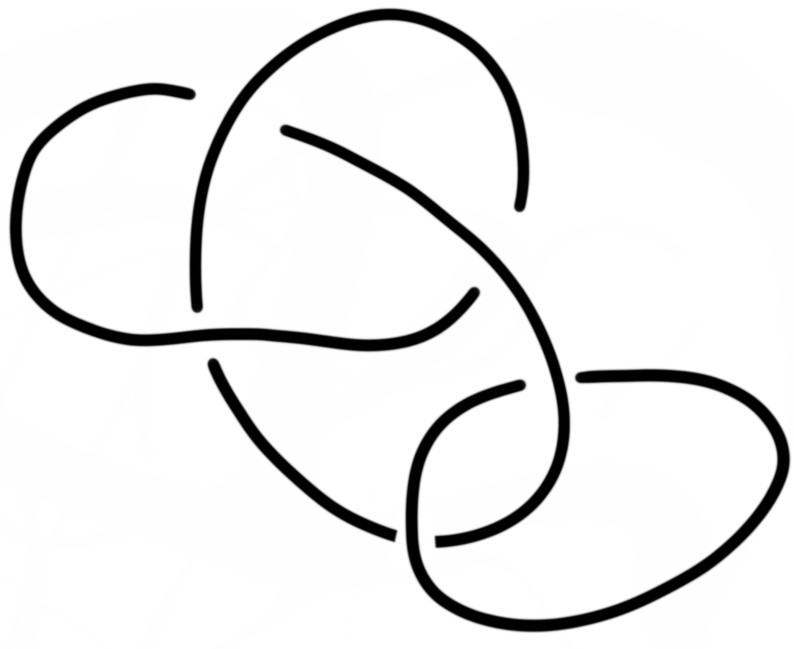
\includegraphics[scale=0.2]{figures/link.jpg}
\label{eq:link}
\end{equation}

We say that $L\simeq L'$ if there is a sequence of Reidemeister moves from $L$ to $L'$, i.e. reversible local strand deformations that do not change the topology, for example by cutting or gluing strands (see Appendix).

The Jones polynomial $V_L(t)$
is a Laurent polynomial in $t\in\mathbb{C}$
and is a link \emph{invariant}.
This means that
$V_L(t)\neq V_{L'}(t)\Rightarrow L\not\simeq L'$,
where $L\simeq L'$.

In general, computing $V_L(t)$
is exponentially costly in the number of crossings $|C|$,
something made explicit when one uses the Kauffman bracket method where a skein relation is used iteratively on every crossing [KauffmanBook].
Exactly evaluating the Jones polynomial at specific points $t\in\mathbb{C}$ is \#P-hard.
\emph{except} at the \emph{lattice roots of unity} $\pm 1, \pm i, \pm e^{i 2\pi/3}, \pm e^{i 4\pi/3}$ where it can be evaluated efficiently (in time $O(poly(|C|))$) [Welsh].


In the context of quantum computation,
additively approximating the Jones polynomial at non-lattice roots of unity is the paradigmatic BQP-complete complete problem [aharonov].
For the lattice roots of unity, the quantum amplitude to which the problem reduces can be computed efficiently.
Specifically, the quantum circuits that need to be simulated are stabiliser circuits which are known to be classically tractable [ref? Kuperberg? Aharonov?].
From the more natural point of view of topological quantum computation,
the jones polynomial at roots of unity corresponds to a quantum amplitude in the fusion space of non-abelian anyons.
Computation is performed by initialising, braiding, and the anyons.
Specifically, in the case of $\text{SU}(2)_k$ anyons, the Jones polynomial is evaluated at $e^{i\frac{2\pi}{2+k}}$ [Rowel-Wang]. Note the correspondence $q\in\{1,2,3,4\}\Leftrightarrow k\in{1,2,4}$.
This is consistent with the fact that topological quantum computation with $\text{SU}(2)_2$ anyons (Ising) or $\text{SU}(2)_4$ anyons is not universal (unless the $\text{SU}(2)_4$ anyons are augmented by fusion and measurements in which case they are capable of universal quantum computation [1504.02098]).



Remarkably, the Jones polynomial can be expressed in terms of the partition function of a $q$-state Potts model [Wu].
The Potts model is defined on a signed graph, called the Tait graph, which is obtained as follows.
The link diagram is bicoloured (checkerboard style)
and every coloured area is mapped to a vertex and every crossing is mapped to a signed edge according
its orientation relative to the surrounding colours.
Every vertex is assigned a $q$-state classical spin
and every signed edge indicates a spin-spin Tait-sign-dependent interaction $J_\pm\in\mathbb{C}$ which relate to the Jones polynomial's variable as $e^{J_\pm}=-t^\mp$.
The role of the link invariant is played by the partition function $Z(q)$;
in fact, the interactions $J_\pm$ are such so that the graph operations corresponding to Reidemeister moves leave $Z(q)$ invariant.
Multiplying with an efficiently computatble prefactor $\mathcal{A}(t) = (-t^\frac{1}{2}-t^{-\frac{1}{2}})^{(-|V|-1)} (-t^\frac{3}{4})^w t^{\frac{1}{4}\tau}$ for bookkeeping of twist factors, the relation to the Jones polynomial is
$V_L(t) = \mathcal{A}(t) Z(q)$.
The link shown in Eq.\ref{eq:link} returns the following tensor network.


\begin{equation}
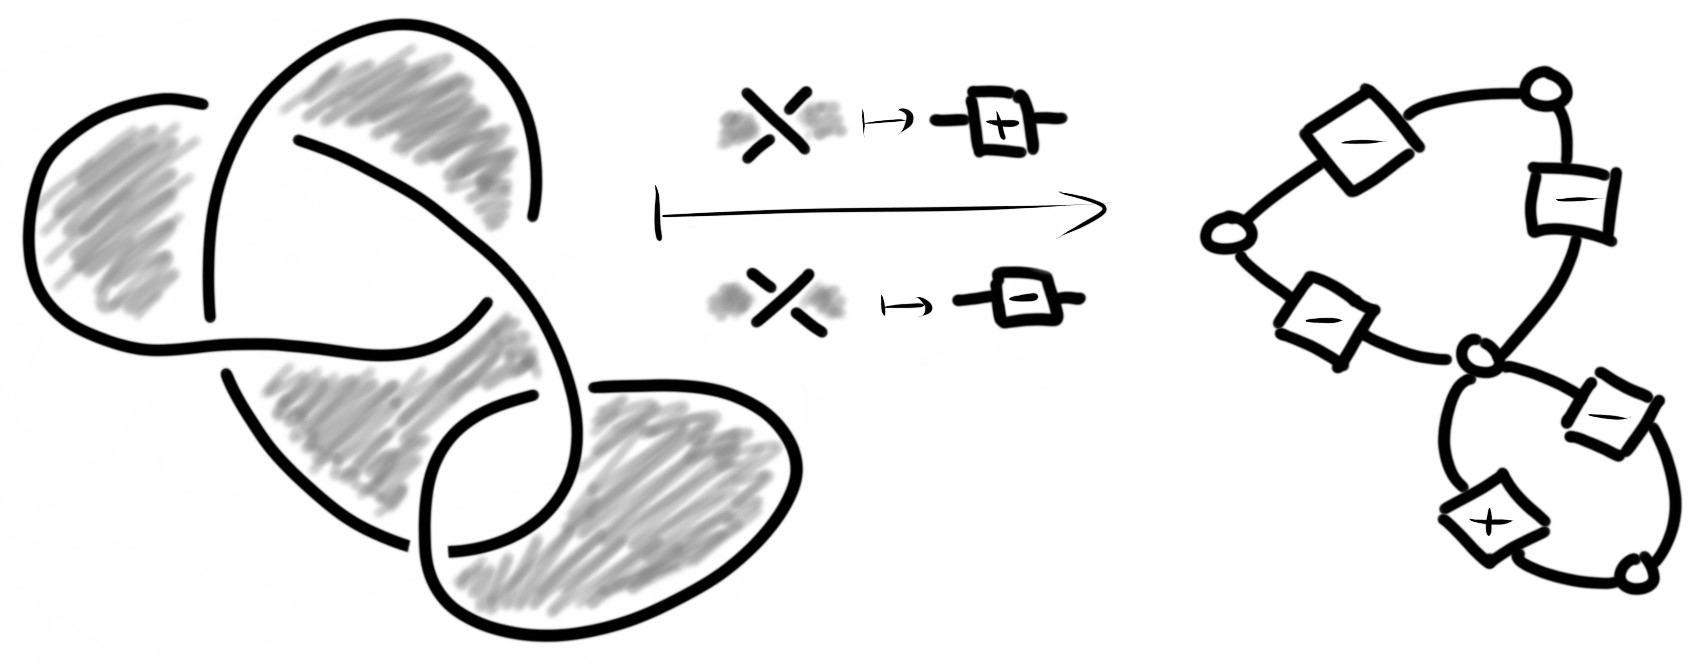
\includegraphics[scale=0.2]{figures/link-tn.jpg}
\label{eq:link-tn}
\end{equation}



For $q=2$ in ZX notation:
\begin{equation}
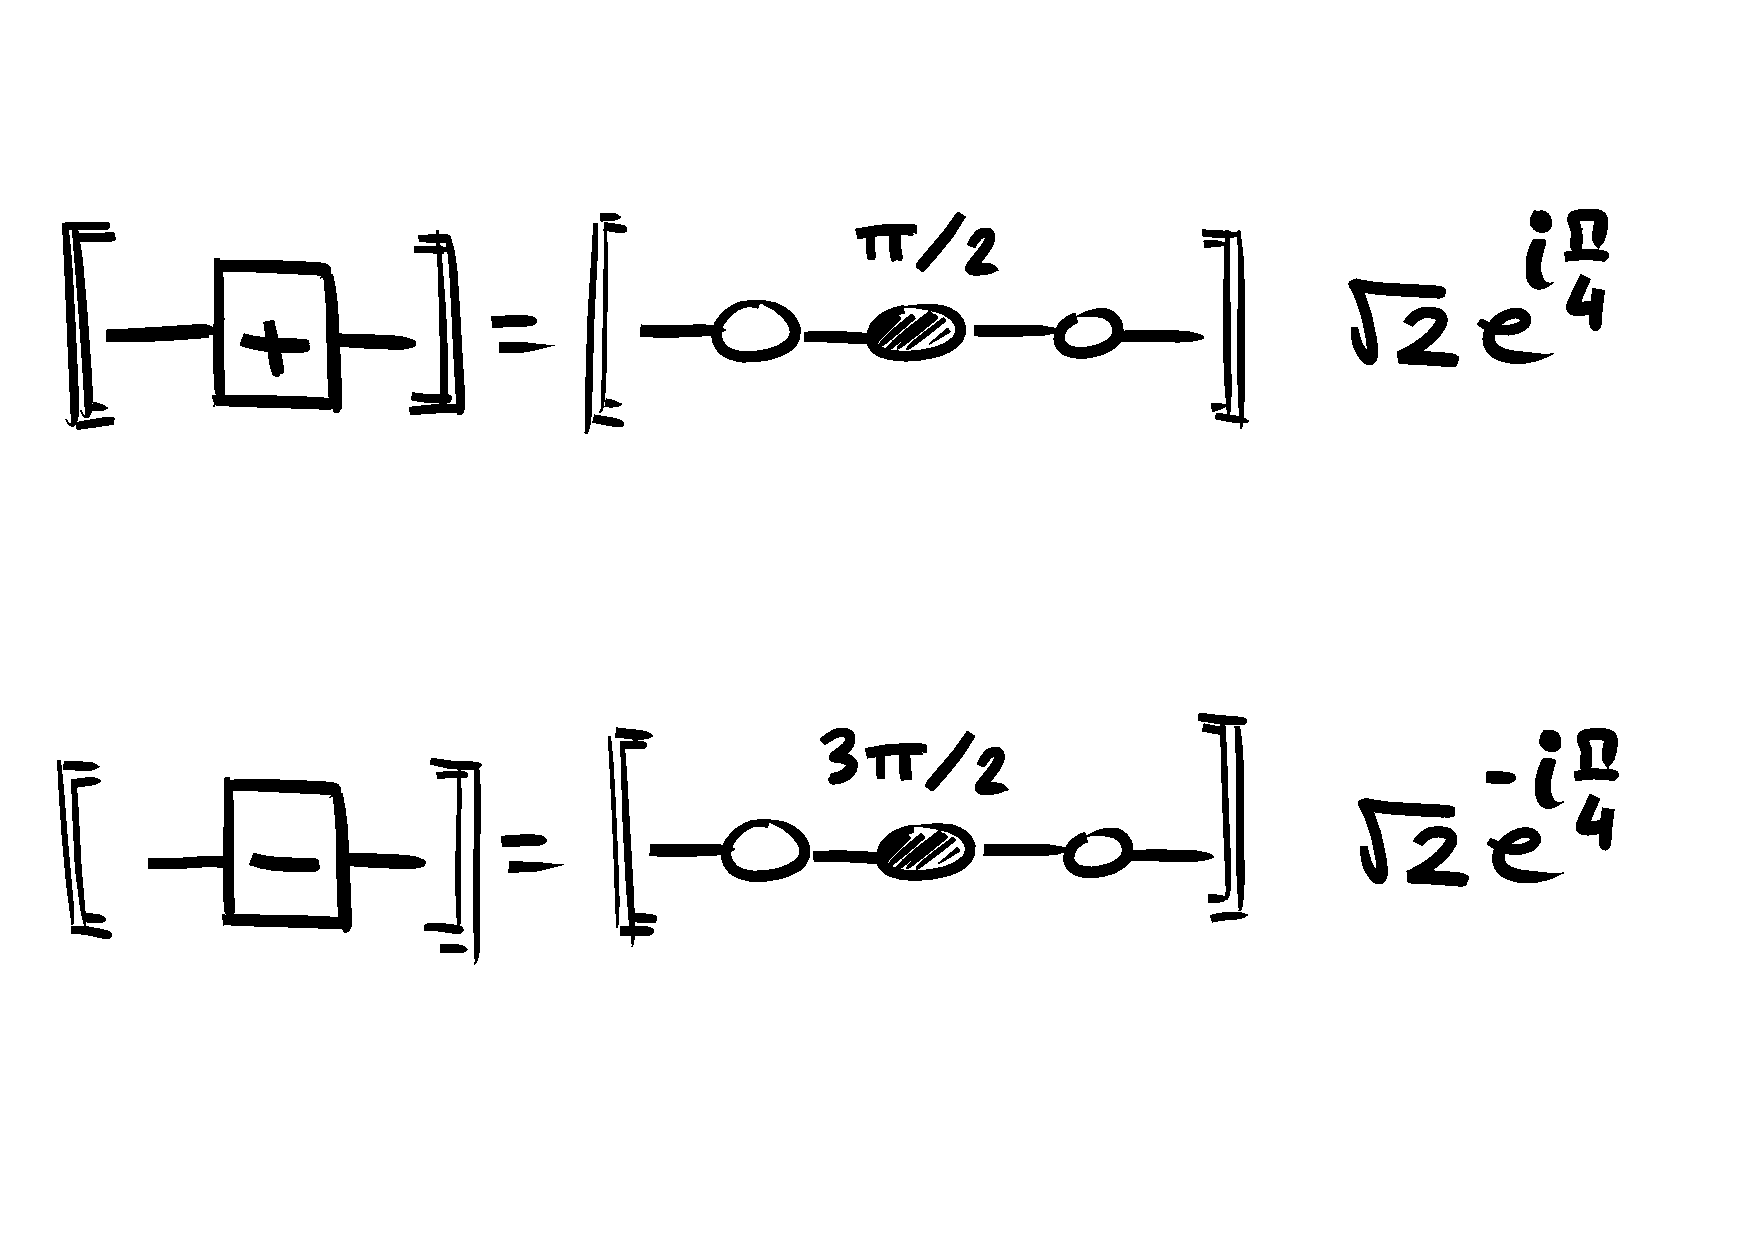
\includegraphics[scale=0.15]{figures/q2.pdf}
\end{equation}





We provide a graphical proof that
evaluating the Jones polynomial of arbitrary links at the lattice roots of unity is in P. For these cases, the problem reduces to the evaluation of the partition function of a planar $q$-state Potts model.
The partition is represented as a closed tensor network.
We employ the ZX-calculus,
which is a sound and complete graphical language
for tensor networks and
allows reasoning via graphical rewrites.
We show that there exist polynomially long rewrite sequences
that fully simplify the tensor network and return $Z(q)$
for $q\in\{1,2,3,4\}$, which correspond to evaluating the Jones polynomial at the lattice roots of unity.


\begin{remark}\label{rem:qubit_scalar_exactness} 
	A small technical remark is in order: the rule set given here is complete for qubit stabilizer quantum mechanics when equality is taken only up to a scalar factor. To achieve completeness under exact equality, a slighly modified rule set would be required, as in (for example) \cite{backens_scalar_exact}. But for our purposes this would be overkill; in order to show that the Jones polynomial of knots at lattice roots of unity is efficiently computable, it suffices to consider the `non-exact' rules - i.e. it suffices to show such a Jones polynomial is efficiently computable up to a scalar factor. But of course to actually compute such a Jones polynomial, we will need to keep track of scalars.
\end{remark}

We can now give ZX-diagrams whose standard interpretations are equal (up to a scalar) to the matrices $T_{\pm}^{(q)}$ in \eqref{eq:pm_tensor} for $q \in \{2, 4\}$.

% [Move commented out stuff below to appendix proof?]

% DON"T DELETE!!!!!!!!!!!!!!!!!!!!!!!
 % This is because the standard interpretation of diagrams more complex than a single spider can be derived as follows. First a diagram is divided into horizontal strips, then these strips are themselves divided vertically, so that the diagram consists of spiders composed in parallel (side-by-side, written $\otimes$) and in sequence (on top of each other, with legs fused together, written $\circ$). Such a division always exists, though it may require a diagram deformation. For example:

For spiders $S$ and $T$, we then have:

\begin{equation}
	\left\llbracket S \otimes T \right\rrbracket = \left\llbracket S \right\rrbracket \otimes \left\llbracket T \right\rrbracket 
\end{equation} 
\begin{equation}	
	\left\llbracket S \circ T \right\rrbracket = \left\llbracket S \right\rrbracket \left\llbracket T \right\rrbracket 
\end{equation} 

where on the right hand side of the first equation the $\otimes$ symbol means the Kronecker product of two matrices. Thus a diagram with standard interpretation $T_{2\pm}$ will have one input and one output, while a diagram for $T_{4\pm}$ will have two inputs and two outputs.

\begin{proposition}\label{prop:pm_map_q2_q4}
	Under the standard interpretation as linear maps, the following diagrams give (up to a scalar) the required matrices:
	\begin{equation}
		\left\llbracket \ \tikzfig{pm_maps/q2} \ \right\rrbracket \simeq \left\llbracket \ \tikzfig{pm_maps/pm} \ \right\rrbracket_{q=2} , 
		\qquad\quad
		\left\llbracket \ \tikzfig{pm_maps/q4} \ \right\rrbracket \simeq \left\llbracket \ \tikzfig{pm_maps/pm} \ \right\rrbracket_{q=4} .
	\end{equation}
	\begin{proof}
		See Appendix \ref{prop:pm_maps_zx_appendix}.
	\end{proof}
\end{proposition}

Since any ZX-diagram derived from a knot in the manner described in Section \ref{sec:passage} will be closed, this algorithm suffices to prove that the calculation of the Jones polynomial of any knot at the lattice roots of unity $\pm 1$ and $\pm i$ is efficient. This is because reading off the scalar at the end is trivial; either we have the empty diagram, which has standard interpretation $1$, or a single legless $Z$-spider with phase $k\pi$:

\begin{equation}
	\left\llbracket \ \tikzfig{scalars/Z_kpi_1} \ \right\rrbracket = 
	\left\llbracket \ \tikzfig{scalars/Z_kpi_2} \ \right\rrbracket = 
	( \bra{0} + \bra{1} )( \ket{0} + e^{ik\pi}\ket{1} ) =
	1 + e^{ik\pi}
\end{equation}

Furthermore, keeping track of the scalar factors introduced with each application of Theorem \ref{thm:qubit_eliminate_spiders} or Lemma \ref{lem:2_h_edges_vanish} can be done efficiently. [ToDo: proof, if not explicitly doing all this in a scalar-exact fashion. Reference Backens]


Having now defined the qutrit ZX-calculus we turn our attention back to our tensor network for the Jones polynomial of a knot (ToDo: ref). We are seeking a diagram in the qutrit ZX-calculus that equals (up to a scalar) the matrix $T_{\pm}^{(q)}$ from \eqref{eq:pm_tensor}.

% where we have used $t = \frac{1}{2}(3 - 2 + \sqrt{3(3-4)}) = e^{i\frac{\pi}{3}}$ as in (ToDo: ref). 

\begin{proposition}\label{prop:pm_map_q3}
	Under the standard interpretation as a linear map, the following diagram gives (up to a scalar) the required matrix:
	\begin{equation}
		\left\llbracket \quad \tikzfig{pm_maps/q3} \quad \right\rrbracket \simeq
		% 2\sqrt{3}e^{\mp i\frac{5\pi}{6}} \ 
		\left\llbracket \quad \tikzfig{pm_maps/pm} \quad \right\rrbracket_{q=3} = 
		\begin{pmatrix}
			e^{\mp i\frac{\pi}{3}} & 1 & 1 \\
			1 & e^{\mp i\frac{\pi}{3}} & 1 \\
			1 & 1 & e^{\mp i\frac{\pi}{3}} \\
		\end{pmatrix}
	\end{equation}

	\begin{proof}
		See Appendix \ref{prop:pm_maps_zx_appendix}.
	\end{proof}
\end{proposition}

Crucially, the ZX-diagram in Proposition \ref{prop:pm_map_q3} above is a \textit{stabilizer diagram} in the qutrit ZX-calculus - that is, all angles are integer multiples of $\frac{2\pi}{3}$. Therefore if we can find an algorithm analogous to Theorem 5.4 \cite{graph_theoretic_simplification} that efficiently reduces any stabilizer diagram to a trivial one, then we will have shown that the Jones polynomial of any knot at the lattice roots of unity $\pm e^{i\frac{\pi}{3}}$ is efficiently computable. [ToDo: justify the $\pm$]. In the next subsection, we will do exactly that.

% Again - just like in Remark~\ref{rem:qubit_scalar_exactness} - these rules are complete for qutrit stabilizer quantum mechanics when equality is considered only up to a scalar factor; we give the scalar-exact versions (detailed in \citep{qutrit_exact}) so that we can actually compute Jones polynomials later. 

\subsection{Graph Colouring}


\section{Outlook}


This also motivates further work in circuit extraction for qutrit circuits so that one can attempt graph-theoretic simplification with the qutrit ZX calculus, analogous to the case of qubits \cite{graph_theoretic_simplification,backens2020again}.
{\bf harny's crazy generalisations: what can they potentially do for general CSP?}


Future work, scalar exact version of the qutrit rewrite rules,
for concrete applications to problems where $3$-state systems are involved.
Further,
generalisation of local complementation and pivot rewrites to arbitrary prime dimension.
Software implementations a la pyzx could be extended accordingly.



\section{Acknowledgments}
Alex would like to thank Aleks Kissinger and Quanlong (Harny) Wang for their help throughout this research.
KM wishes to thank Niel de Beaudrap, Aleks Kissinger, Stefanos 
Kourtis, and Quanlong (Harny) Wang for inspiring and helpful discussions.
KM acknowledges financial support from the Royal Commission for the Exhibition of 1851 through a research fellowship.





\bibliographystyle{eptcs}
\bibliography{refs-teague,refs}

% \section{Appendix}

We begin with proofs of the translations of the matrix $T_{\pm}^{(q)}$ into the ZX-calculus. 

\begin{proposition}\label{prop:pm_maps_zx_appendix} \textbf{/\ Propositions~\ref{prop:pm_map_q2_q4}, \ref{prop:pm_map_q3}.}
	The following equalities hold up to a scalar under the standard interpretation:
	\begin{equation*}
		\left\llbracket \ \tikzfig{pm_maps/q2} \ \right\rrbracket \simeq \left\llbracket \ \tikzfig{pm_maps/pm} \ \right\rrbracket_{q=2} \ , \qquad
		\left\llbracket \ \tikzfig{pm_maps/q3} \ \right\rrbracket \simeq \left\llbracket \ \tikzfig{pm_maps/pm} \ \right\rrbracket_{q=3} \ , \quad
		\left\llbracket \ \tikzfig{pm_maps/q4} \ \right\rrbracket \simeq \left\llbracket \ \tikzfig{pm_maps/pm} \ \right\rrbracket_{q=4}
	\end{equation*}

	\begin{proof}
		Recalling $\omega = e^{i\frac{2\pi}{3}}$, the standard interpretations of phase gates in matrix form are:
		
		\begin{equation*}
			\left\llbracket \ \tikzfig{pm_maps/qubit/Z_phase} \ \right\rrbracket = 
			\begin{pmatrix}
				1 & 0 \\
				0 & e^{i\alpha}
			\end{pmatrix} \ , \quad
			\left\llbracket \ \tikzfig{pm_maps/qubit/X_phase} \ \right\rrbracket = 
			\frac{1}{2} \begin{pmatrix}
				1 + e^{i\alpha} & 1 - e^{i\alpha} \\
				1 - e^{i\alpha} & 1 + e^{i\alpha}
			\end{pmatrix} \ , \quad
			\left\llbracket \ \tikzfig{pm_maps/qutrit/Z_phase} \ \right\rrbracket = 
			\begin{pmatrix}
				1 & 0 & 0\\
				0 & e^{i\alpha} & 0 \\
				0 & 0 & e^{i\beta}
			\end{pmatrix}
		\end{equation*}
		\begin{equation*}
			\left\llbracket \ \tikzfig{pm_maps/qutrit/X_phase} \ \right\rrbracket = 
			\frac{1}{3} \begin{pmatrix}
				1 + e^{i\alpha} + e^{i\beta} & 1 + \bar{\omega}e^{i\alpha} + {\omega}e^{i\beta} & 1 + {\omega}e^{i\alpha} + \bar{\omega}e^{i\beta} \\
				1 + {\omega}e^{i\alpha} + \bar{\omega}e^{i\beta} & 1 + e^{i\alpha} + e^{i\beta} & 1 + \bar{\omega}e^{i\alpha} + {\omega}e^{i\beta} \\
				1 + \bar{\omega}e^{i\alpha} + {\omega}e^{i\beta} & 1 + {\omega}e^{i\alpha} + \bar{\omega}e^{i\beta} & 1 + e^{i\alpha} + e^{i\beta} \\
			\end{pmatrix}
		\end{equation*}

		So in the simplest case $q=2$ it is fairly straightforward to see that:

		\begin{equation}
			\left\llbracket \ \tikzfig{pm_maps/q2} \ \right\rrbracket \ = \ 
			\frac{1}{2} \begin{pmatrix}
				1 \pm i & 1 \mp i \\
				1 \mp i & 1 \pm i \\
			\end{pmatrix} \ = \ 
			\frac{\sqrt{2}}{2} e^{\mp i \frac{\pi}{4}} \begin{pmatrix}
				\pm i & 1 \\
				1 & \pm i \\
			\end{pmatrix} \ = \ 
			\frac{\sqrt{2}}{2} e^{\mp i \frac{\pi}{4}} \left\llbracket \ \tikzfig{pm_maps/pm} \ \right\rrbracket_{q=2}
		\end{equation}

		The next case $q=3$ is proved similarly:

		\begin{equation}
		\begin{aligned}
				\left\llbracket \ \tikzfig{pm_maps/q3} \ \right\rrbracket
				&= \frac{1}{3} \begin{pmatrix}
					1 + e^{\pm i\frac{2\pi}{3}} + e^{\pm i\frac{2\pi}{3}} & 1 + \bar{\omega}e^{\pm i\frac{2\pi}{3}} + {\omega}e^{\pm i\frac{2\pi}{3}} & 1 + {\omega}e^{\pm i\frac{2\pi}{3}} + \bar{\omega}e^{\pm i\frac{2\pi}{3}} \\
					1 + {\omega}e^{\pm i\frac{2\pi}{3}} + \bar{\omega}e^{\pm i\frac{2\pi}{3}} & 1 + e^{\pm i\frac{2\pi}{3}} + e^{\pm i\frac{2\pi}{3}} & 1 + \bar{\omega}e^{\pm i\frac{2\pi}{3}} + {\omega}e^{\pm i\frac{2\pi}{3}} \\
					1 + \bar{\omega}e^{\pm i\frac{2\pi}{3}} + {\omega}e^{\pm i\frac{2\pi}{3}} & 1 + {\omega}e^{\pm i\frac{2\pi}{3}} + \bar{\omega}e^{\pm i\frac{2\pi}{3}} & 1 + e^{\pm i\frac{2\pi}{3}} + e^{\pm i\frac{2\pi}{3}} \\
				\end{pmatrix} \\
				&= \frac{1}{3} \begin{pmatrix}
					\sqrt{3}e^{\pm i\frac{\pi}{2}} & \sqrt{3}e^{\mp i\frac{\pi}{6}} & \sqrt{3}e^{\mp i\frac{\pi}{6}} \\
					\sqrt{3}e^{\mp i\frac{\pi}{6}} & \sqrt{3}e^{\pm i\frac{\pi}{2}} & \sqrt{3}e^{\mp i\frac{\pi}{6}} \\
					\sqrt{3}e^{\mp i\frac{\pi}{6}} & \sqrt{3}e^{\mp i\frac{\pi}{6}} & \sqrt{3}e^{\pm i\frac{\pi}{2}} \\
				\end{pmatrix} \\
				&= \frac{\sqrt{3}}{3} e^{\mp i\frac{\pi}{6}}\begin{pmatrix}
					e^{\pm i\frac{2\pi}{3}} & 1 & 1 \\
					1 & e^{\pm i\frac{2\pi}{3}} & 1 \\
					1 & 1 & e^{\pm i\frac{2\pi}{3}} \\
				\end{pmatrix} \\
				&= \frac{\sqrt{3}}{3} e^{\mp i\frac{\pi}{6}} \left\llbracket \ \tikzfig{pm_maps/pm} \ \right\rrbracket_{q=3}
			\end{aligned}
		\end{equation}

		For the other qubit case $q=4$ we first note:

		\begin{equation}
			\left\llbracket \ \tikzfig{qubit_hadamard/yellow_box} \ \right\rrbracket = 
			\left\llbracket \ \tikzfig{qubit_hadamard/decomposed} \ \right\rrbracket =
			\left\llbracket \ \qubitZphase{\frac{\pi}{2}} \ \right\rrbracket
			\left\llbracket \ \qubitXphase{\frac{\pi}{2}} \ \right\rrbracket
			\left\llbracket \ \qubitZphase{\frac{\pi}{2}} \ \right\rrbracket = 
			\frac{1}{2\sqrt{2}} \begin{pmatrix}
				1 & 1 \\
				1 & -1 \\
			\end{pmatrix}
		\end{equation}

		Then using the standard interpretation for spiders (Definition \ref{def:qubit_standard_spiders}) we decompose the diagram in such a way that we can apply the standard interpretation:

		\begingroup
			\allowdisplaybreaks
				\begin{align*}
					\left\llbracket \ \tikzfig{pm_maps/q4} \ \right\rrbracket 
					&= \left\llbracket \ \tikzfig{pm_maps/q4/decomposed} \ \right\rrbracket \\
					&= \left(
						\left\llbracket \ \tikzfig{pm_maps/q4/id} \ \right\rrbracket \otimes 
						\left\llbracket \ \tikzfig{pm_maps/q4/pi_compare} \ \right\rrbracket
					\right)
					\left(
						\left\llbracket \ \tikzfig{pm_maps/q4/id} \ \right\rrbracket \otimes 
						\left\llbracket \ \tikzfig{pm_maps/q4/hadamard} \ \right\rrbracket \otimes 
						\left\llbracket \ \tikzfig{pm_maps/q4/id} \ \right\rrbracket 
					\right)
					\left(
						\left\llbracket \ \tikzfig{pm_maps/q4/pi_copy} \ \right\rrbracket \otimes 
						\left\llbracket \ \tikzfig{pm_maps/q4/id} \ \right\rrbracket
					\right) \\
					&= \frac{\sqrt{2}}{8} \begin{pmatrix}
						-1 & 1 & 1 & 1 \\
						1 & -1 & 1 & 1 \\
						1 & 1 & -1 & 1 \\
						1 & 1 & 1 & -1 \\
					\end{pmatrix} \\
					&= \frac{\sqrt{2}}{8} \left\llbracket \ \tikzfig{pm_maps/pm} \ \right\rrbracket_{q=4}
				\end{align*}
		\endgroup
	\end{proof}
\end{proposition}

Next we prove the local pivot equality from Theorem~\ref{thm:local_pivot_equality}. For this, recall that all but the $\qutritRuleCommute$ and $\qutritRuleColourChange$ qutrit rewrite rules hold under taking adjoints, and with the roles of green and red swapped, so in particular rule $\qutritRuleEuler$ also gives:

\begin{equation}\label{eq:qutrit_hadamard_decompositions}
	\tikzfig{qutrit_rules/hadamard/euler/h} = \tikzfig{qutrit_rules/hadamard/euler/decomposition} \ , \hspace{50pt} 
	\tikzfig{qutrit_rules/hadamard/euler/h} = \tikzfig{hadamard_lemmas/decompositions/h} \ , \hspace{50pt} 
	\tikzfig{hadamard_lemmas/decompositions/h_dagger} = \tikzfig{hadamard_lemmas/decompositions/h_dagger_xzx} \ , \hspace{50pt}
	\tikzfig{hadamard_lemmas/decompositions/h_dagger} = \tikzfig{hadamard_lemmas/decompositions/h_dagger_zxz} \
\end{equation}

\begin{theorem}\label{thm:local_pivot_equality_appendix} \textbf{/\ Theorem~\ref{thm:local_pivot_equality}.} 
	Given $a \in \mathbb{Z}_3$ and a graph state $(G, W)$ containing connected nodes $i$ and $j$, define the following:
	\begin{itemize}
		\item $N_{=}(i, j) \defeq \left\{k \in N(i) \cap N(j) \mid w_{k,i} = w_{k,j} \right\}$
		\item $N_{\neq}(i, j) \defeq \left\{k \in N(i) \cap N(j) \mid w_{k,i} \neq w_{k,j} \right\}$
	\end{itemize} 
	Then the following equation relates $G$ and its proper $a$-local pivot along $ij$:
	\ctikzfig{graph_state/proper_local_pivot}
	\begin{proof}
		Annoyingly, proving this in full generality in one go - i.e. for a proper $a$-local pivot along an edge $ij$ of weight $b$ - becomes a bit tricky diagramatically, because it becomes hard to keep track of all the variable edge weights. Fortunately the four cases ($a, b \in \{1,2\}$) split into two pairs of symmetric cases: $a = b$ and $a \neq b$.\newline

		Now, it suffices to only draw a fragment of a graph state. Certainly we consider nodes $i$ and $j$ and the edge $ij$ between them. Then define $N_x^y$ to be the set $\left\{k \mid w_{k,i} = x, w_{k,j} = y \right\}$, for $x, y, \in \mathbb{Z}_3$. We will consider a representative node $k_x^y$ from each $N_x^y \neq N_0^0$, as well as its edges $ik_x^y$ and $jk_x^y$. All other nodes and edges are irrelevant; this is because we are only interested in nodes and edges that \textit{affect} the three local complementation operations on $i$ and $j$ - we aren't concerned with those that are only \textit{affected by} the operations.\newline

		So for the case $a=b$, we show the proper $1$-local pivot along $ij$ of weight $1$:

		\begingroup
			\allowdisplaybreaks
			\setlength{\jot}{20pt}
			\begin{align*}
				&\ &&\tikzfig{proper_1_local_pivot/weight_1/step_1} 
				&&&\xeq{\ref{thm:local_comp_equality}} 
				&&&&\tikzfig{proper_1_local_pivot/weight_1/step_2} \\
				&\xeq{\ref{thm:local_comp_equality}} 
				&&\tikzfig{proper_1_local_pivot/weight_1/step_3} 
				&&&\xeq{\ref{thm:local_comp_equality}} 
				&&&&\tikzfig{proper_1_local_pivot/weight_1/step_4} \\
				&\xeqq{\eqref{eq:qutrit_hadamard_decompositions}}{\qutritRuleFusion} 
				&&\tikzfig{proper_1_local_pivot/weight_1/step_5} 
				&&&= &&&&\tikzfig{proper_1_local_pivot/weight_1/step_6} \\
			\end{align*}
		\endgroup

		The story is similar for the case $a \neq b$; here we show the proper $1$-local pivot along $ij$ of weight $2$:

		\begingroup
			\allowdisplaybreaks
			\setlength{\jot}{20pt}
			\begin{align*}
				&\ &&\tikzfig{proper_1_local_pivot/weight_2/step_1} 
				&&&\xeq{\ref{thm:local_comp_equality}} 
				&&&&\tikzfig{proper_1_local_pivot/weight_2/step_2} \\
				&\xeq{\ref{thm:local_comp_equality}} 
				&&\tikzfig{proper_1_local_pivot/weight_2/step_3} 
				&&&\xeq{\ref{thm:local_comp_equality}} 
				&&&&\tikzfig{proper_1_local_pivot/weight_2/step_4} \\
				&\xeqq{\eqref{eq:qutrit_hadamard_decompositions}}{\qutritRuleFusion} 
				&&\tikzfig{proper_1_local_pivot/weight_2/step_5} 
				&&&= &&&&\tikzfig{proper_1_local_pivot/weight_2/step_6} \\
			\end{align*}
		\endgroup

		% \ctikzfig{proper_1_local_pivot_weight_2_line_1}
		% \ctikzfig{proper_1_local_pivot_weight_2_line_2}
		% \ctikzfig{proper_1_local_pivot_weight_2_line_3}

		The case $a=b=2$ is the same as $a=b=1$, except with the roles of purple and blue edges interchanged, so by symmetry of the diagram the only difference is in the phase gates added to the outputs. Namely, on each phase gate we replace all instances of $1$ with a $2$. Thus the roles of $H$ and $H^\dagger$ are swapped too. Likewise for the case $(a,b) = (2,1)$ with respect to the case $(a,b) = (1,2)$.

	\end{proof}
\end{theorem}

Now we prove the three elimination theorems for $\mathcal{M}$-, $\mathcal{N}$- and \Pspiders. First, we require two lemmas.

\begin{lemma}\label{lem:leg_flip}
	The following `leg flip' equation holds in the qutrit ZX-calculus. Moreover, it holds with the roles of green and red swapped.
	\begin{equation*}
		\tikzfig{leg_flip/1} = \tikzfig{leg_flip/5}
	\end{equation*}
	\begin{proof}
		\begin{equation*}
			\tikzfig{leg_flip/1} \ \xeq{\qutritRuleFusion} \ 
			\tikzfig{leg_flip/2} \ \xeq{\qutritRuleSnake} \ 
			\tikzfig{leg_flip/3} \ \xeq{\qutritRuleColourChange} \  
			\tikzfig{leg_flip/4} \ \xeq{\qutritRuleColourChange} \  
			\tikzfig{leg_flip/5}
		\end{equation*}
	\end{proof}
\end{lemma}

\begin{lemma}\label{lem:substantial_m_copy}
	The following more substantial `$\mathcal{M}$-copy' rule holds in the qutrit ZX-calculus, for any \Mspider\ state (i.e. $m \in \{0, 1, 2\}$ below). Moreover, it holds with the roles of green and red swapped.
	\begin{equation*}
		\tikzfig{m_copies/full/1} = \tikzfig{m_copies/full/4}
	\end{equation*}
	\begin{proof}
		First we prove that an \Mspider\ with non-trivial phase (i.e. $m \in \{1, 2\}$) satisfies a copy rule exactly like the rule $\qutritRuleZeroCopy$:
		\begin{equation}\label{eq:non_trivial_m_copy}
			\tikzfig{m_copies/part_1/1} \ \xeq{\qutritRuleFusion} \ 
			\tikzfig{m_copies/part_1/2} \ \xeq{\qutritRuleMCopy} \ 
			\tikzfig{m_copies/part_1/3} \ \xeq{\qutritRuleZeroCopy} \ 
			\tikzfig{m_copies/part_1/4} \ \xeq{\qutritRuleFusion} \ 
			\tikzfig{m_copies/part_1/5}
		\end{equation}
		Then we prove the case $\alpha = \beta = 0$ by induction:
		\begin{equation}\label{eq:m_copy_through_trivial}
			\tikzfig{m_copies/part_2/1} \ \xeq{\qutritRuleFusion} \ 
			\tikzfig{m_copies/part_2/2} \ \xeq{\eqref{eq:non_trivial_m_copy}} \ 
			\tikzfig{m_copies/part_2/3} \ \xeq{\text{ind.}} \ 
			\tikzfig{m_copies/part_2/4}
		\end{equation}
		Which finally allows us to prove the full statement, where the last equality is just dropping the scalar term:
		\begin{equation*}
			\tikzfig{m_copies/full/1} \ \xeq{\qutritRuleFusion} \ 
			\tikzfig{m_copies/full/2} \ \xeq{\eqref{eq:m_copy_through_trivial}} \ 
			\tikzfig{m_copies/full/3} \ = \
			\tikzfig{m_copies/full/4}
		\end{equation*}
	\end{proof}
\end{lemma}

We are now in a position to prove the \Mspider\ elimination theorem.

\begin{theorem}\label{thm:eliminate_M_spiders_appendix} \textbf{/\ Theorem~\ref{thm:eliminate_M_spiders}.}
	Given any graph-like ZX-diagram containing two interior \Mspiders\ $i$ and $j$ connected by edge $ij$ of weight $w_{i,j} \eqdef w \in \{1,2\}$, suppose we perform a proper $\pm w$-local pivot along $ij$. Then the new ZX-diagram is related to the old one by the equality:
	
	\ctikzfig{eliminate/M_spiders/theorem_LHS}
	\ctikzfig{eliminate/M_spiders/theorem_RHS}
	
	where all changes to weights of edges where neither endpoint is $i$ or $j$ are omitted. Furthermore, in order to save space, each node with phase \qutritZphase{a_x^y}{b_x^y} is representative of \textit{all} nodes connected to $i$ by an $x$-weighted edge and to $j$ by a $y$-weighted edge.

	\begin{proof}
		We show the case where $w_{ij} \eqdef w = 1$, with the case $w = 2$ being completely analogous. We can choose either a proper $1$-local pivot or a proper $2$-local pivot; both give the same result. Here we only show the former:
		\begingroup
			\allowdisplaybreaks
			\setlength{\jot}{30pt}
			\begin{align*}
				&\ &&\tikzfig{eliminate/M_spiders/step_1} \\
				&\xeq{\qutritRuleFusion} 
				&&\tikzfig{eliminate/M_spiders/step_2} \\
				&\xeq{\ref{thm:local_pivot_equality_appendix}} 
				&&\tikzfig{eliminate/M_spiders/step_3} \\
				&\xeq{\qutritRuleColourChange}
				&&\tikzfig{eliminate/M_spiders/step_4} \\
				&\xeq{\ref{lem:leg_flip}}
				&&\tikzfig{eliminate/M_spiders/step_5} \\
				&\xeq{\ref{lem:substantial_m_copy}}
				&&\tikzfig{eliminate/M_spiders/step_6} \\
				&= 
				&&\tikzfig{eliminate/M_spiders/step_7} \\
				&\xeq{\qutritRuleColourChange}
				&&\tikzfig{eliminate/M_spiders/step_8} \\
				&\xeq{\qutritRuleFusion}
				&&\tikzfig{eliminate/M_spiders/step_9} \\
			\end{align*}
		\endgroup
	\end{proof}
\end{theorem}

Proving the corresponding \Nspider\ elimination theorem requires a further lemma, which allows us to turn an \Nspider\ state of one colour into an \Nspider\ state of the other.

\begin{lemma}\label{lem:N_state_colour_change}
	The following rules hold in the qutrit ZX-calculus:
	\begin{equation*}
		\tikzfig{n_states/0_1/z} \ = \ \tikzfig{n_states/0_1/x} \ , \qquad
		\tikzfig{n_states/0_2/z} \ = \ \tikzfig{n_states/0_2/x} \ , \qquad
		\tikzfig{n_states/1_0/z} \ = \ \tikzfig{n_states/1_0/x} \ , \qquad
		\tikzfig{n_states/2_0/z} \ = \ \tikzfig{n_states/2_0/x}
	\end{equation*}
	\begin{proof}
		The key observation is that for any green \Nspider\ state with phase $\qutritZphase{n}{n'}$, we have a choice of two colour change rules which we could use to turn it into a red \Nspider\ state with a $H$- or $H^\dagger$-box on top:
		
		\begin{equation*}
			\tikzfig{n_states/general/x_n_n'} \ \xeq{\qutritRuleColourChange} \ 
			\tikzfig{n_states/general/z_n_n'} \ \xeq{\qutritRuleColourChange} \ 
			\tikzfig{n_states/general/x_n'_n}
		\end{equation*}

		Of these two choices, exactly one has a decomposition of of the $H$-/$H^\dagger$-box as in \eqref{eq:qutrit_hadamard_decompositions} that allows the bottom two red spiders to fuse into an \Mspider, which we can then move past the green spider above it via \ref{lem:substantial_m_copy}. For brevity we only show the case $\qutritZphase{n}{n'} = \qutritZphase{0}{1}$:

		\begin{equation*}
			\tikzfig{n_states/0_1/1} \ \ \xeq{\qutritRuleColourChange} \ \ 
			\tikzfig{n_states/0_1/2} \ \ \xeq{\eqref{eq:qutrit_hadamard_decompositions}} \ \ 
			\tikzfig{n_states/0_1/3} \ \ \xeq{\qutritRuleFusion} \ \ 
			\tikzfig{n_states/0_1/4} \ \ \xeq{\ref{lem:substantial_m_copy}} \ \ 
			\tikzfig{n_states/0_1/5} \ \ \xeq{\qutritRuleFusion} \ \ 
			\tikzfig{n_states/0_1/6}
		\end{equation*}
	\end{proof}
\end{lemma}

\begin{corollary}\label{cor:N_effect}
	The following equations hold in the qutrit ZX-calculus:
	\begin{equation*}
		\tikzfig{n_states/corollary/0_n/lhs} \ = \ \tikzfig{n_states/corollary/0_n/rhs} \ , \qquad
		\tikzfig{n_states/corollary/n_0/lhs} \ = \ \tikzfig{n_states/corollary/n_0/rhs}
	\end{equation*}
	\begin{proof}
		Again we only prove one case, the rest being analogous. Each case uses \ref{lem:N_state_colour_change} in its adjoint form - recall that the adjoint of a spider is found by swapping inputs and outputs and negating angles.
		\begin{equation*}
			\tikzfig{n_states/corollary/0_1/1} \ \ = \ \ 
			\tikzfig{n_states/corollary/0_1/2} \ \ \xeq{\ref{lem:N_state_colour_change}} \ \ 
			\tikzfig{n_states/corollary/0_1/3} \ \ \xeq{\qutritRuleFusion} \ \ 
			\tikzfig{n_states/corollary/0_1/4} \ \ = \ \ 
			\tikzfig{n_states/corollary/0_1/5}
		\end{equation*}
	\end{proof}
\end{corollary}

\begin{theorem}\label{thm:eliminate_N_spiders_appendix} \textbf{/\ Theorem~\ref{thm:eliminate_N_spiders}.}
	Given any graph-like ZX-diagram containing an interior \Nspider\ $k$ with phase \qutritZphase{0}{n} for $n \in \{1,2\}$, suppose we perform a $(-n)$-local complementation at $k$. Then the new ZX-diagram is related to the old one by the equality:

	\begin{equation*}
		\tikzfig{eliminate/N_spiders/0_n/step_1} \quad = \quad \tikzfig{eliminate/N_spiders/0_n/step_9}
	\end{equation*}

	where all changes to weights of edges where neither endpoint is $k$ are omitted. If instead $k$ has phase \qutritZphase{n}{0} for $n \in \{1,2\}$, suppose we perform the same $(-n)$-local complementation at $k$. Then the equality relating the new and old diagrams becomes:

	% Spiders with phases \qutritZphase{a_1}{b_1} ... \qutritZphase{a_r}{b_r} are all the neighbours of $k$ connected by a $1$-weighted (blue) edge, while spider with phases \qutritZphase{c_1}{d_1} ... \qutritZphase{c_s}{d_s} are all the neighbours of $k$ connected by a $2$-weighted (purple) edge.\newline

	\begin{equation*}
		\tikzfig{eliminate/N_spiders/n_0/step_1} \quad = \quad \tikzfig{eliminate/N_spiders/n_0/step_9}
	\end{equation*}

	\begin{proof}
		We prove the case where $k$ has phase \qutritZphase{0}{n} for $n \in \{1,2\}$, the other case being near-identical.
		\begingroup
			\allowdisplaybreaks
			\setlength{\jot}{20pt}
				\begin{align*}
					&\ &&\tikzfig{eliminate/N_spiders/0_n/step_1} 
					&&&\xeq{\qutritRuleFusion} 
					&&&&\tikzfig{eliminate/N_spiders/0_n/step_2} \\
					&\xeq{\ref{thm:local_comp_equality}} 
					&&\tikzfig{eliminate/N_spiders/0_n/step_3} 
					&&&\xeqq{\ref{cor:N_effect}}{\qutritRuleFusion} 
					&&&&\tikzfig{eliminate/N_spiders/0_n/step_4} \\
					&\xeq{\ref{lem:leg_flip}} 
					&&\tikzfig{eliminate/N_spiders/0_n/step_5} 
					&&&\xeq{\ref{lem:substantial_m_copy}} 
					&&&&\tikzfig{eliminate/N_spiders/0_n/step_6} \\
					&\xeq{\eqref{eq:qutrit_dashed_lines}}
					&&\tikzfig{eliminate/N_spiders/0_n/step_7} 
					&&&\xeq{\qutritRuleColourChange} 
					&&&&\tikzfig{eliminate/N_spiders/0_n/step_8} \\
					&\xeq{\qutritRuleFusion} 
					&&\tikzfig{eliminate/N_spiders/0_n/step_9} \\
				\end{align*}
		\endgroup
	\end{proof}
\end{theorem}

Similarly the corresponding \Pspider\ elimination theorem requires a lemma allowing us to turn a \Pspider\ state of one colour into a \Pspider\ state of the other. As above, we will use this lemma its adjoint form in the proof of the main theorem.

\begin{lemma}\label{lem:P_state_colour_change}
	The following rule holds in the qutrit ZX-calculus:
	\begin{equation*}
		\tikzfig{p_state/1} \ = \ \tikzfig{p_state/6}
	\end{equation*}
	\begin{proof}
		The proof structure is exactly as in \ref{lem:N_state_colour_change}, only for \Pspiders\ it's even simpler:
		\begin{equation*}
			\tikzfig{p_state/1} \ \ \xeq{\qutritRuleColourChange} \ \ 
			\tikzfig{p_state/2} \ \ \xeq{\eqref{eq:qutrit_hadamard_decompositions}} \ \ 
			\tikzfig{p_state/3} \ \ \xeq{\qutritRuleFusion} \ \ 
			\tikzfig{p_state/4} \ \ \xeq{\ref{lem:substantial_m_copy}} \ \ 
			\tikzfig{p_state/5} \ \ \xeq{\qutritRuleFusion} \ \ 
			\tikzfig{p_state/6}
		\end{equation*}
	\end{proof}
\end{lemma}

\begin{theorem}\label{thm:eliminate_P_spiders_appendix} \textbf{/\ Theorem~\ref{thm:eliminate_P_spiders}.} 
	Given any graph-like ZX-diagram containing an interior \Pspider\ $k$ with phase \qutritZphase{p}{p} for $p \in \{1,2\}$, suppose we perform a $p$-local complementation at $k$. Then the new ZX-diagram is related to the old one by the equality:

	\begin{equation*}
		\tikzfig{eliminate/P_spiders/step_1} \quad = \quad \tikzfig{eliminate/P_spiders/step_9}
	\end{equation*}

	where all changes to weights of edges where neither endpoint is $k$ are omitted. 

	\begin{proof}
		\begingroup
			\allowdisplaybreaks
			\setlength{\jot}{20pt}
				\begin{align*}
					&\ &&\tikzfig{eliminate/P_spiders/step_1} 
					&&&\xeq{\qutritRuleFusion} 
					&&&&\tikzfig{eliminate/P_spiders/step_2} \\
					&\xeq{\ref{thm:local_comp_equality}} 
					&&\tikzfig{eliminate/P_spiders/step_3} 
					&&&\xeqq{\ref{lem:P_state_colour_change}}{\qutritRuleFusion} 
					&&&&\tikzfig{eliminate/P_spiders/step_4} \\
					&\xeq{\ref{lem:leg_flip}} 
					&&\tikzfig{eliminate/P_spiders/step_5} 
					&&&\xeq{\ref{lem:substantial_m_copy}} 
					&&&&\tikzfig{eliminate/P_spiders/step_6} \\
					&\xeq{\eqref{eq:qutrit_dashed_lines}}
					&&\tikzfig{eliminate/P_spiders/step_7} 
					&&&\xeq{\qutritRuleColourChange} 
					&&&&\tikzfig{eliminate/P_spiders/step_8} \\
					&\xeq{\qutritRuleFusion} 
					&&\tikzfig{eliminate/P_spiders/step_9} \\
				\end{align*}
		\endgroup
	\end{proof}
\end{theorem}

\end{document} 